\chapter{Unlabeled Data Utilization through Semi-Supervised Learning}

\section{Introduction}

The abundance of unlabeled data in real-world scenarios presents both a challenge and an opportunity for modern machine learning systems and, critically, for foundation models. While supervised learning methods have achieved remarkable success, their reliance on large quantities of labeled data limits their applicability in domains where annotation is costly, time-consuming, or impractical. Semi-supervised learning (SSL) addresses this limitation by leveraging the vast pool of unlabeled data alongside a small set of labeled examples, enabling models to learn more robust and generalizable representations—precisely the data efficiency required for foundation model deployment.

For wireless foundation models, semi-supervised learning serves two essential purposes. First, it provides a practical training methodology that reduces the labeled data requirements during the pre-training stage (Chapter 2), allowing models like DenoMAE to learn from massive unlabeled signal datasets with minimal supervision. Second, it enables efficient fine-tuning during the adaptation stage (Chapter 3), where meta-learning techniques can be enhanced with semi-supervised objectives to maximize utilization of available unlabeled signals in deployment environments.

This chapter explores advanced semi-supervised learning techniques designed to maximize the utility of unlabeled data, with particular focus on their application in classification tasks. We discuss the theoretical foundations of SSL, review state-of-the-art methods such as pseudo-labeling, consistency regularization, and self-supervised pretext tasks, and highlight their strengths and limitations in data-constrained environments. Furthermore, we introduce \textbf{RLPL (Representation Learning with Pseudo-Labeling)}—our novel approach that integrates improved representation learning and pseudo-labeling strategies, demonstrating effectiveness in enhancing classification accuracy and generalization with limited labeled data.

Through comprehensive experiments and analysis, we show how the proposed methods bridge the gap between supervised and unsupervised learning, offering practical solutions for scenarios where labeled data is scarce but unlabeled data is plentiful. For wireless foundation models, this paradigm is critical: spectrum monitoring generates continuous streams of unlabeled signals, but obtaining expert-labeled modulation classifications at scale is prohibitively expensive. RLPL enables foundation models to learn effectively from this imbalanced data distribution.

\textbf{Foundation Model Context:} This chapter complements Chapters 2 and 3 by providing the practical training methodology that makes wireless foundation models viable. Chapter 2 introduced self-supervised pre-training (Stage 1); Chapter 3 introduced meta-learning for rapid adaptation (Stage 2); this chapter demonstrates how semi-supervised learning enhances both stages by maximizing unlabeled data utilization. Together, these techniques enable the three-stage wireless foundation model framework: (1) pre-train on unlabeled signals via masked autoencoders, (2) adapt rapidly with meta-learning using small labeled sets augmented by semi-supervised objectives, and (3) integrate with LLMs for open-set recognition (Chapter 5). The insights and techniques presented in this chapter contribute to developing flexible, data-efficient machine learning frameworks capable of adapting to a wide range of real-world wireless challenges.

\subsection{Semi-Supervised Learning: An Overview}

At its core, semi-supervised learning seeks to improve model performance beyond what is achievable with the limited labeled data alone by exploiting the information latent within the abundant unlabeled data. The fundamental principle is that the structure, patterns, or underlying distribution of the unlabeled data ($p(x)$) contains valuable information about the target function, specifically the conditional probability of the label given the input ($p(y|x)$). Labeled data points serve to ground the model's predictions, establishing the number of classes and their basic characteristics, while the unlabeled data provides crucial context about the overall shape and density of the data distribution, helping to refine decision boundaries.

The typical mechanism involves an initial learning phase where the model is trained on the small labeled dataset using conventional supervised techniques. Subsequently, the model leverages the unlabeled data, often in an iterative fashion, to refine its understanding and improve predictions. This refinement process varies depending on the specific SSL algorithm. For instance, when processing labeled data points, the algorithm updates model parameters using traditional supervised loss functions that compare predictions to true labels. For unlabeled data points, the objective often shifts to minimizing the difference in predictions between similar unlabeled points or enforcing consistency in predictions under various perturbations.

The primary motivation behind the development and adoption of SSL stems from a fundamental challenge in practical machine learning: the data labeling bottleneck. Acquiring large datasets is often feasible and relatively inexpensive, especially with the proliferation of digital data sources. However, annotating this data with accurate labels typically requires significant human effort, domain expertise, time, and financial resources. This disparity between the ease of collecting unlabeled data and the difficulty of labeling it creates a scenario where vast amounts of potentially useful data remain underutilized by purely supervised methods. SSL directly addresses this imbalance, offering a pathway to potentially achieve performance comparable to fully supervised models but with a substantially reduced labeling requirement. The economic pressure to reduce annotation costs while still building high-performance models makes SSL not merely a technical curiosity but often an economic imperative in data-rich, label-poor environments. Its relevance is thus intrinsically linked to the practicalities and economics of data acquisition in the real world, growing in importance as data generation continues to outpace annotation capabilities.

A crucial prerequisite for successful SSL is the relevance of the unlabeled data to the learning task. Formally, the distribution of the input data, $p(x)$, as revealed by the unlabeled examples, must contain information about the posterior distribution $p(y|x)$. Using unlabeled data that is unrelated to the target classes (e.g., training a cat/dog classifier with unlabeled images of vehicles) will not improve performance and may even degrade it.


% TODO: add a figure for SSL.

SSL techniques can be broadly categorized into several groups:

\begin{itemize}
    \item \textbf{Generative Methods:} These approaches model the joint probability distribution of data and labels, using both labeled and unlabeled data to estimate the underlying structure. Examples include generative adversarial networks (GANs) and variational autoencoders (VAEs) adapted for SSL. By learning the data distribution, generative models can synthesize new samples or infer missing labels, providing additional supervision for the learning process. These methods are particularly effective when the data distribution is complex and high-dimensional, as in image or text domains.

    \item \textbf{Self-Training and Pseudo-Labeling:} In these methods, a model trained on labeled data is used to assign pseudo-labels to unlabeled samples. The model is then retrained using both true and pseudo-labeled data, iteratively refining its predictions. This approach leverages the model's own confidence to expand the labeled dataset, but care must be taken to avoid reinforcing incorrect predictions. Techniques such as confidence thresholding and ensembling are often used to improve the reliability of pseudo-labels.

    \item \textbf{Consistency Regularization:} These techniques encourage the model to produce consistent predictions for unlabeled data under different perturbations or augmentations. Methods such as Mean Teacher, Virtual Adversarial Training (VAT), and FixMatch fall into this category. The underlying assumption is that the model's output should be invariant to small changes in the input, promoting smoother decision boundaries. Consistency regularization has proven highly effective in computer vision tasks, where data augmentations are easy to define.

    \item \textbf{Graph-Based Methods:} These approaches represent data as nodes in a graph, propagating label information from labeled to unlabeled nodes based on their similarity or connectivity. Graph-based SSL leverages the manifold structure of the data, assuming that similar samples are likely to share the same label. Techniques such as label propagation and graph convolutional networks (GCNs) are commonly used, especially in applications involving relational or networked data.

    \item \textbf{Self-Supervised Pretext Tasks:} Here, auxiliary tasks are designed to learn useful representations from unlabeled data, which can then be transferred to the main supervised task. Examples include predicting image rotations, solving jigsaw puzzles, or reconstructing masked input features. By solving these pretext tasks, models learn to extract semantic features from data without explicit labels, improving downstream performance when labeled data is limited.
\end{itemize}

The effectiveness of SSL depends on several assumptions, such as the cluster assumption (data points in the same cluster are likely to share a label) and the smoothness assumption (similar inputs have similar outputs). When these assumptions hold, SSL can significantly boost performance compared to purely supervised approaches.

\section{Related Work}
In this section, we review key developments in semi-supervised learning, focusing on major approaches and methodologies that have shaped the field. We examine how different techniques leverage unlabeled data to improve model performance, particularly in scenarios with limited labeled data availability.

\subsection{Contrastive Learning}

Contrastive learning has emerged as a powerful framework for self-supervised representation learning, achieving remarkable success across various domains, particularly computer vision. This approach learns representations by optimizing a contrastive objective that attracts semantically similar (positive) pairs while repelling dissimilar (negative) pairs in an embedding space~\cite{chen2020simple}. In vision applications, positive pairs typically comprise augmented views of the same image, whereas negative pairs consist of different images.

Early contrastive methods faced scalability challenges due to their reliance on large numbers of negative examples to avoid representational collapse. SimCLR~\cite{chen2020simple} demonstrated strong performance but required large batch sizes (4,096+) to provide sufficient negative examples, imposing substantial computational demands. MoCo~\cite{he2020momentum} addressed this limitation through a momentum encoder and a dynamic queue of negative samples, effectively decoupling training batch size from the number of negative examples and enabling more efficient training on standard hardware.

The contrastive learning paradigm has been extended to multimodal and sequential domains with significant success. CLIP~\cite{radford2021learning} scaled contrastive learning to 400 million image-text pairs, creating aligned visual and textual representations that enable remarkable zero-shot transfer to downstream tasks. In sequential data modeling, Contrastive Predictive Coding (CPC)~\cite{oord2018representation} predicts future representations in latent space using a contrastive objective, capturing temporal dependencies across modalities including speech, images, and text.

Despite their empirical success, contrastive methods face fundamental limitations. The quality of learned representations depends critically on the sampling strategy for negative pairs and the design of data augmentations, which often require domain-specific knowledge. Additionally, the binary notion of similarity (positive/negative) may not capture complex semantic relationships, and the requirement for many negative examples can introduce sampling bias or computational inefficiency.

Recent research has explored alternatives to address these challenges, including hard negative mining~\cite{robinson2020contrastive}, learnable data augmentation~\cite{morerio2024model}, and hybrid approaches that combine contrastive objectives with other self-supervised signals. PiCO~\cite{wang2022pico} extend contrastive learning to partially labeled data by incorporating prototype-based objectives, while others leverage contrastive pre-trained models to identify reliable pseudo-labels for unlabeled data. These developments highlight contrastive learning's importance in the broader semi-supervised learning ecosystem, particularly for label-efficient fine-tuning.

\subsection{Representation Learning}

Representation learning forms the cornerstone of modern semi-supervised approaches by transforming raw data into meaningful feature spaces where downstream tasks become more tractable. Central to this paradigm is the manifold hypothesis~\cite{whiteley2022statistical}, which posits that high-dimensional data typically concentrates near lower-dimensional structures. Learning these manifolds enables models to disentangle important factors of variation while discarding noise, creating representations where the smoothness and cluster assumptions of SSL become more applicable~\cite{sohn2020fixmatch}.

Non-contrastive approaches address limitations of negative sampling by employing alternative objectives. BYOL~\cite{grill2020bootstrap} uses a teacher-student framework with a momentum-updated target network and successfully learns representations without negative examples. Similarly, SimSiam~\cite{chen2020exploring} demonstrates that even simpler architectures without momentum encoders can avoid representational collapse through careful use of stop-gradients and prediction heads. Redundancy reduction methods take yet another approach. Barlow Twins~\cite{zbontar2021barlow} minimizes redundancy between representation dimensions by making the cross-correlation matrix between two augmented views approach the identity matrix. This elegantly addresses both alignment and uniformity aspects of representation learning without requiring negative samples or momentum networks.

For sequential data, specialized methods have emerged. Wav2Vec~\cite{baevski2020wav2vec} and its successors learn representations from raw audio by predicting future encodings in latent space, enabling breakthrough performance in speech recognition with limited labeled data. These approaches demonstrate how representation learning can be adapted to the unique characteristics of different data modalities. Generative approaches offer a complementary perspective. Masked Autoencoders~\cite{he2022masked} learn representations by reconstructing images from heavily masked inputs, showing that predicting missing content creates powerful visual features that transfer well to downstream tasks. Earlier variants like Denoising Autoencoders~\cite{vincent2008extracting} and Variational Autoencoders~\cite{kingma2013auto} similarly learn representations through reconstruction objectives.

Graph Neural Networks (GNNs) extend representation learning to non-Euclidean data by learning node embeddings that capture both node features and graph topology through message-passing operations~\cite{kipf2016semi, hamilton2017inductive}. These approaches have enabled semi-supervised learning on relational data where traditional methods struggle.

The effectiveness of these representation learning techniques in semi-supervised scenarios stems from their ability to leverage unlabeled data to discover data manifolds that align with downstream task boundaries. When these learned representations capture the underlying semantic structure of the data, even simple classifiers can achieve strong performance with limited labeled examples~\cite{oliver2018realistic}. This principle has driven the common two-stage approach of unsupervised pre-training followed by supervised fine-tuning that dominates modern semi-supervised learning.

\subsection{Consistency-Based Learning}

Consistency regularization has emerged as a cornerstone approach in modern semi-supervised learning, founded on the smoothness assumption that a model's predictions should remain invariant under reasonable perturbations of the input or model parameters~\cite{oliver2018realistic,sohn2020fixmatch}. These methods leverage unlabeled data by enforcing consistency between predictions of different views of the same instance, effectively expanding decision boundaries away from high-density regions without requiring explicit labels~\cite{chapelle2009semi}.

Early consistency-based methods established the fundamental paradigm through various perturbation strategies. The Pi-Model~\cite{sajjadi2016regularization} applies stochastic augmentation and dropout, penalizing differences between predictions from two forward passes of the same sample. Temporal Ensembling~\cite{laine2016temporal} extends this by maintaining an exponential moving average (EMA) of past predictions to create more stable targets, reducing variance but introducing delayed feedback. Mean Teacher~\cite{tarvainen2017mean} addresses this limitation by averaging model weights rather than predictions, creating a teacher model that generates targets for the student model, enabling immediate consistency training with every batch.

Adversarial perturbation approaches like Virtual Adversarial Training(VAT)~\cite{miyato2017virtual} generate worst-case perturbations within a norm-constrained neighborhood that maximally change model predictions, enforcing local Lipschitz continuity and improving robustness to adversarial examples. These methods are particularly effective in high-dimensional spaces where random perturbations might fail to challenge the model.

Data augmentation has proven especially powerful for consistency regularization in visual domains. Unsupervised Data Augmentation (UDA)~\cite{xie2019unsupervised} employs strong augmentations like RandAugment for unlabeled data while maintaining consistency with weakly-augmented versions. FixMatch~\cite{sohn2020fixmatch} combines this insight with pseudo-labeling, using confident predictions from weakly-augmented images as targets for strongly-augmented views, creating a simple yet highly effective framework that has become a foundation for numerous subsequent approaches.

Interpolation-based methods further enrich the consistency learning landscape. MixMatch~\cite{berthelot2019mixmatch} introduces a holistic approach that combines temperature sharpening of pseudo-labels with MixUp augmentation applied across both labeled and unlabeled samples. ReMixMatch~\cite{berthelot2019remixmatch} enhances this framework with distribution alignment between pseudo-labels and labeled data, and incorporates an auxiliary self-supervised rotation prediction task to improve feature learning.

Recent advances have focused on adaptive mechanisms that adjust consistency training dynamically. FlexMatch~\cite{zhang2021flexmatch} introduces curriculum learning by adaptively setting confidence thresholds for each class based on learning status, addressing class imbalance issues in pseudo-labeling. CoMatch~\cite{li2021comatch} integrates contrastive learning with consistency training by aligning both prediction-level and representation-level consistencies through a unified graph-based framework. Curriculum Consistency Training (CCT)~\cite{liu2024curriculum} employs multiple auxiliary heads trained with progressively stronger augmentations, creating a natural curriculum that improves robustness.

Beyond conventional training, consistency principles have been extended to test-time adaptation scenarios. Test-Time Training (TTT)~\cite{sun2024learning} applies self-supervised consistency losses during inference to adapt models to distribution shifts without requiring labels, demonstrating the versatility of consistency regularization beyond traditional SSL.

The consistent success of these approaches across diverse tasks and architectures highlights consistency regularization as a fundamental principle in modern machine learning that effectively leverages unlabeled data. Current research continues to explore combinations with other learning paradigms and applications to new domains, suggesting that consistency-based methods will remain central to semi-supervised learning advances.

\subsection{Pseudo Labeling}

In semi-supervised learning, pseudo-labeling is used on a highly accurate classifier to label and learn from it. This approach has proven effective in various applications like object detection \cite{li2022rethinking,yan2019semi}, image classification \cite{taherkhani2021self,wu2017semi}, and speech recognition \cite{lugosch2022pseudo}. If pseudo labels are inaccurately assigned, classifiers may learn from erroneous labels, diminishing their performance \cite{arazo2020pseudo}.

Many pseudo-labeling methods focus on enhancing the network through consistency loss \cite{zhang2021flexmatch}, moving away from the traditional approach of retraining the model with pseudo labels \cite{iscen2019label}. Consistency-based methods ensure stable model predictions across various augmented views of the same input \cite{rizve2021defense}. However, consistency loss typically updates the network with a fraction of the cross-entropy loss \cite{wang2023kd}, reducing its impact. This diminished emphasis on consistency loss can hinder the network's optimal update, as it does not fully leverage retraining with pseudo labels \cite{xie2020unsupervised}.

MPL addresses the issue of incorrect pseudo-labeling by applying a meta-learning \cite{lee2019meta} approach. In MPL, the teacher uses its softmax predictions on unlabeled data to instruct the student. These predictions, commonly called soft labels, are a well-established concept in the literature on knowledge distillation \cite{cho2019efficacy,phuong2019towards}. This additional adaptation empowers the teacher to generate more accurate pseudo labels for instructing the student network. MPL employs the same bi-level optimization technique from meta-learning \cite{snell2017prototypical, nichol2018reptile, finn2017model} to iteratively update the teacher-student framework. Additionally, introducing a controlled noise in either the teacher or student network is helpful, especially when the two networks are similar. This noise injection boosts the learning process's robustness and generalization \cite{wang2023consistent, li2024nicest}.

\section{Preliminaries}

This section introduces the foundational concepts and notations relevant to semi-supervised learning, with a focus on representation learning methods and pseudo-labeling strategies.

\subsection{Problem Setup}

Let $\mathcal{D}_L = \{(x_i, y_i)\}_{i=1}^{N_L}$ denote a labeled dataset, where $x_i \in \mathcal{X}$ are input samples and $y_i \in \mathcal{Y}$ are their corresponding labels. Let $\mathcal{D}_U = \{u_j\}_{j=1}^{N_U}$ denote a much larger set of unlabeled samples, where $u_j \in \mathcal{X}$. The goal of semi-supervised learning is to leverage both $\mathcal{D}_L$ and $\mathcal{D}_U$ to train a model $f_\theta$ that generalizes well to unseen data.

\subsection{Representation Learning with Two-Network Architectures}

Modern semi-supervised representation learning methods often employ two-network architectures, such as the teacher-student or online-target frameworks. Prominent examples are BYOL~\cite{grill2020bootstrap}, Barlow Twins~\cite{zbontar2021barlow}, SimSiam~\cite{chen2020exploring} which consist of:

\begin{itemize}
    \item \textbf{Online Network:} Parameterized by $\theta$, this network receives an augmented view of an input and produces a representation.
    \item \textbf{Target Network:} Parameterized by $\xi$, this network receives a different augmented view of the same input. Its parameters are updated as an exponential moving average (EMA) of the online network: $\xi \leftarrow \tau \xi + (1-\tau)\theta$, where $\tau \in [0,1)$ is the EMA decay rate.
\end{itemize}

The training objective encourages the online network's output to predict the target network's output for the same input under different augmentations, without requiring negative samples. This approach avoids representational collapse and enables effective use of unlabeled data by learning invariant and discriminative features.

\subsection{Pseudo-Labeling}

Pseudo-labeling is a widely used technique in semi-supervised learning where the model generates artificial labels for unlabeled data. The process typically involves:

\begin{enumerate}
    \item Training a model on labeled data $\mathcal{D}_L$.
    \item Using the trained model to predict labels (pseudo-labels) for samples in $\mathcal{D}_U$.
    \item Selecting high-confidence predictions (e.g., those with maximum softmax probability above a threshold) as pseudo-labels.
    \item Retraining or fine-tuning the model using both labeled and pseudo-labeled data.
\end{enumerate}

Variants such as Mean Teacher~\cite{tarvainen2017mean} and Meta Pseudo Labels (MPL)~\cite{lee2019meta} further refine this process by employing teacher-student frameworks, soft labels, and meta-learning strategies. The use of EMA for teacher updates and noise injection for regularization are common practices to improve stability and generalization.

\subsection{Notation Summary}

\begin{itemize}
    \item $\mathcal{D}_L$: Labeled dataset
    \item $\mathcal{D}_U$: Unlabeled dataset
    \item $f_\theta$: Model parameterized by $\theta$
    \item $\xi$: Target/teacher network parameters (EMA of $\theta$)
    \item $\tau$: EMA decay rate
    \item $\hat{y}$: Pseudo-label assigned to an unlabeled sample
\end{itemize}

These preliminaries provide the basis for understanding the advanced semi-supervised learning methods.

\section{Proposed Methodology: Maximizing Unlabeled Data Utility with Improved Representation Learning and Pseudo Labeling}

An effective semi-supervised approach for representation learning involves two parallel networks - a trainable network and a momentum network. Two augmented versions of the input images go through these networks to predict their outputs and thereby learn the representation. However, this method often fails to maximize its full potential. We identify two major issues regarding data utilization: (1) the need for large batch sizes, which reduces efficiency in memory-constrained environments, and (2) the exclusion of unlabeled data during downstream tasks. We address these limitations with a two-step approach. First, we incorporate both original and augmented images into the trainable network and add a weighted loss term to enhance learning with the additional input. After pre-training, pseudo labels are generated in a meta-learning setup using two identical teacher-student networks, where the teacher network progressively outperforms the student by receiving feedback from it. Our approach, Representation Learning with Pseudo Labeling (RLPL), improves representation learning by achieving higher accuracy for half the batch size of existing methods. RLPL demonstrates an average performance gain of \textbf{6.12\%} across the STL-10, CIFAR-10, and SVHN datasets, with individual improvements ranging from  \textbf{2.7\%} to \textbf{15.74\%}.

\subsection{Introduction}


While supervised machine learning algorithms thrive on labeled data, manually annotating this data can be both time-consuming and costly. In contrast, unlabeled data is often readily available and abundant. Although it lacks explicit labels,  unlabeled data still holds valuable information that machine learning models can harness. Semi-supervised learning bridges this gap by extracting meaningful patterns from unlabeled data, compensating for the limited labeled datasets \cite{kingma2014semi}. It achieves this by utilizing the unlabeled data to uncover latent representations—underlying structures and relationships that aren't directly observable. Semi-supervised learning can enhance model performance by incorporating these latent representations, even when labeled data is scarce \cite{devillers2024semi, kutuzova2021multimodal}.

Contrastive learning \cite{chuang2020debiased, fan2023contrastive} has been proven effective in learning the data representation using the unlabeled sample. However, they require negative samples to avoid representational collapse \cite{aghajanyan2020better} and hence were plagued by the problem of mining negative samples \cite{radenovic2023filtering}. There are no apparent methods to obtain effective negative samples, and the presence of higher negative samples than positive ones creates an imbalance \cite{kalantidis2020hard}. Subsequently, contrastive learning methods rely on a large batch size \cite{yang2023batchsampler} to achieve good performance, leading to expensive computational needs.

Representation Learning (RL) methods, such as Bootstrap Your Own Latent (BYOL), SimSiam, and Barlow Twins solve the problem of negative samples by learning representation from the positive class alone. While these methods achieve impressive results with large batch sizes (typically 1024-4096), their performance degrades significantly with smaller batches. This degradation occurs because larger batches provide better gradient estimates and more diverse learning signals, which are crucial for stable representation learning. However, the high memory requirements of large batches make these methods impractical for resource-constrained environments.

Our analysis reveals that the performance drop in existing methods with smaller batches (8-128) stems from two key factors: (1) unstable gradient estimates leading to suboptimal convergence, and (2) limited diversity in the learning signals within each batch. RLPL addresses these challenges through a novel approach that maximizes information utilization from each sample, enabling stable learning even with smaller batches. Through extensive experimentation across different batch sizes, we demonstrate that RLPL maintains consistent performance, showing only a marginal accuracy drop with reduced batch sizes.

Unlabeled data, typically unused in downstream tasks, can enhance performance when leveraged through a model with strong initialization. Pseudo-Labels (PL) \cite{lee2013pseudo} employ a confidence threshold to selectively include those unlabeled samples for which the classifier demonstrates high certainty in its predictions. RL offers an effective initialization, enabling improved model performance and confident pseudo-labeling. However, a notable challenge arises when incorrect pseudo labels are assigned, leading to a degradation in classifier accuracy due to learning from corrupted data. RLPL addresses this issue by refining the pseudo labels through a teacher-student network. This process enhances the teacher network, making it a better model to guide the student network, thereby generating more accurate pseudo labels and boosting overall performance.

Typical RL methods demand extensive computational resources, such as hundreds of TPUs over several days. Additionally, pseudo-labeling is another memory-heavy method as it uses two networks simultaneously. These requirements are challenging in scenarios where fast, efficient models are needed, like in autonomous vehicles or edge computing \cite{guo2023architecture}. To address these limitations, we implement RLPL on a more manageable batch size and a shallower network, leveraging just two Nvidia 4090 GPUs. Our study shows that RLPL, even without the usage of pseudo labeling, achieves higher accuracy with a batch size of 64, outperforming BYOL with a 128 batch size. Remarkably, RLPL consistently outperforms other RLs with a ResNet18 classifier. RLPL yields average accuracy improvements of \textbf{2.7\%}, \textbf{9.22\%}, and \textbf{4.16\%} that the closest contemporary method on the STL-10, CIFAR-10, and SVHN datasets, respectively. Figure \ref{fig:flow} illustrates our proposed framework. Codes are available at \href{https://github.com/atik666/rlpl}{https://github.com/atik666/rlpl}.

\begin{figure*}[!htbp]
    \centering  
    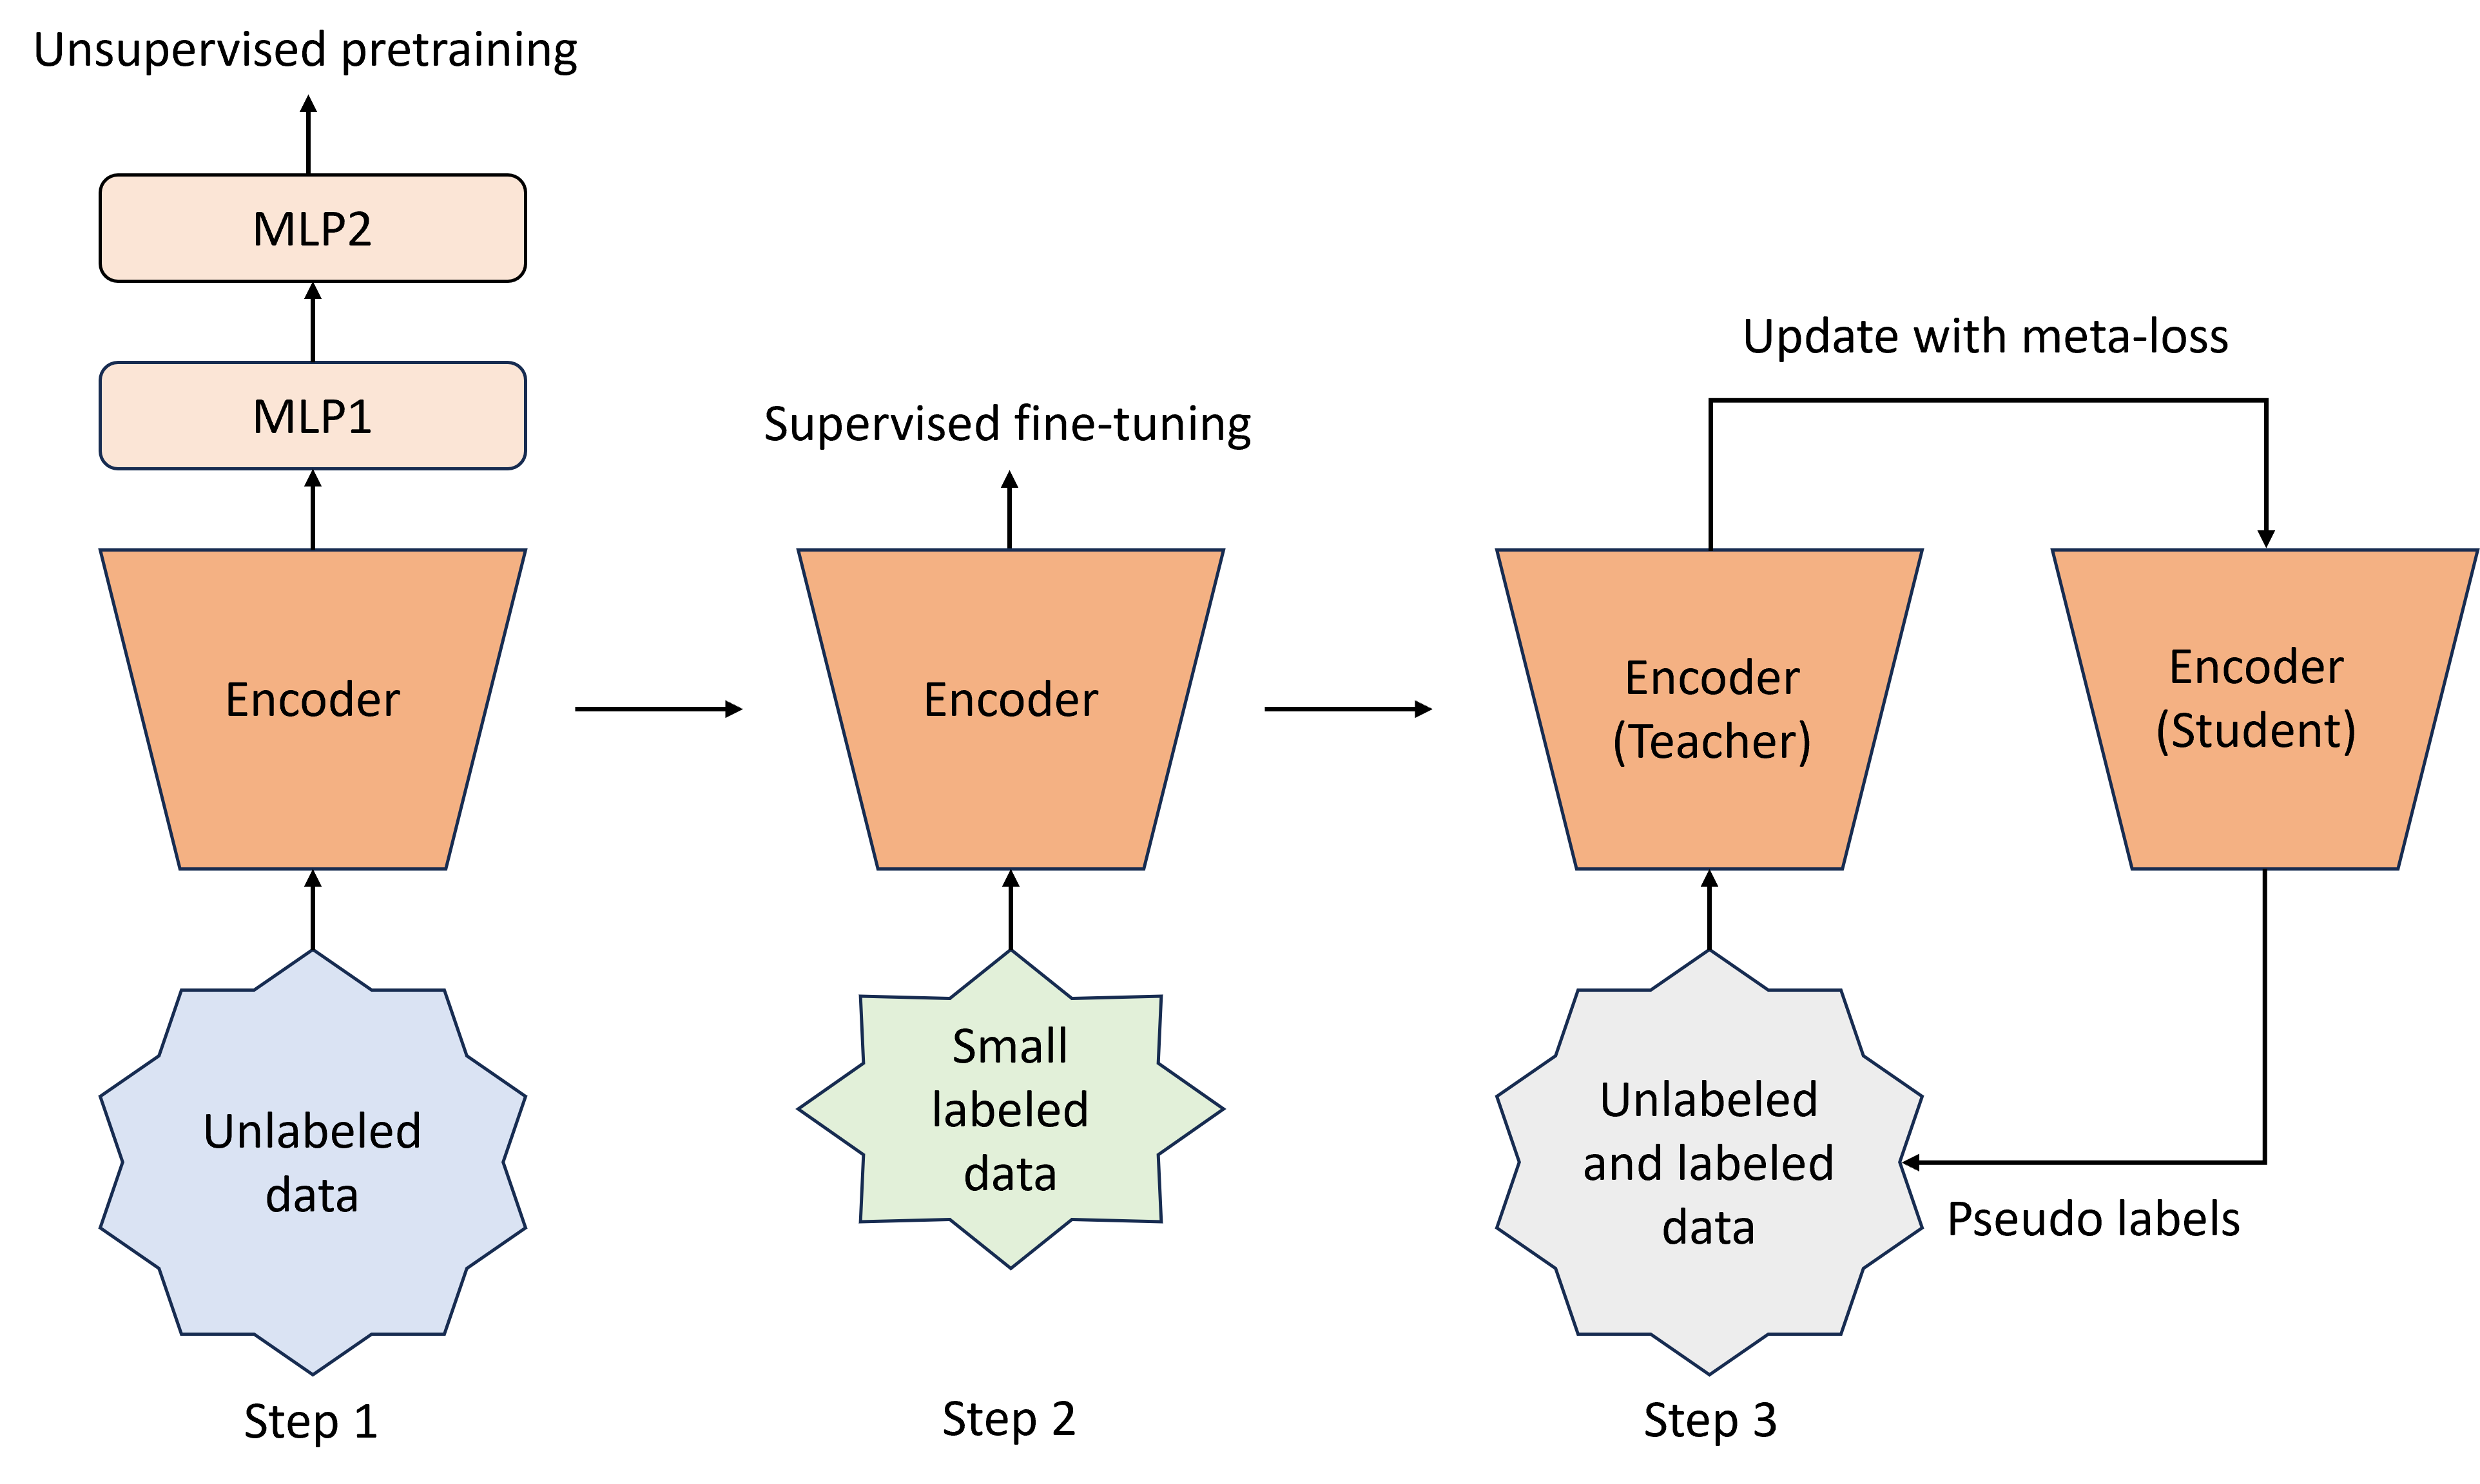
\includegraphics[width=0.9\textwidth]{FIGURES/rlpl/flow.png}
    \caption{\textbf{RLPL flowchart.} 
    RLPL has two levels of unlabeled data utilization. First, it employs unsupervised representation learning. Second, We obtain a highly accurate fine-tuned classifier using only a handful of label data. Lastly, through pseudo labelling using teacher-student networks, both initialized from superior supervised backbone, we improve the classifier further.}
    \label{fig:flow}
\end{figure*}
\section{Introduction}    

\subsection{Contributions}

In summary, our work contains the following contributions:

\begin{itemize}

    \item Our approach cleverly leverages most information from the inputs, leading to enhanced global representation learning. By making this strategic adjustment, our model achieves improved representations with a smaller batch size, ultimately achieving higher accuracy in the downstream tasks.
    
    \item During the downstream task, we utilize unlabeled samples a second time with pseudo labeling. Our approach uses the student network feedback with a meta-loss update to improve the noisy teacher \cite{xie2020self} as the final classifier.
    
    \item RLPL outperforms other State-Of-The-Art (SOTA) RL algorithms on an equivalent but more compact architecture, making it more efficient and cost-effective for edge computing in resource-constrained environments.
    
    \end{itemize}

\subsection{Proposed Methodology: RLPL}

We propose a novel framework, RLPL, effectively utilizes unlabeled data through two key innovations: (1) enhanced representation learning with auxiliary loss functions, and (2) refined pseudo-labeling with meta-learning. This section details the technical aspects of our approach.


\subsubsection{Improved Representation Learning}

In RLPL, the trainable and momentum networks use identical encoders for image embeddings. These embeddings are projected to a lower-dimensional space using a Multi-Layer Perceptron (MLP) in each network. The momentum network stops here, producing outputs with a dimension of 256. In contrast, the trainable network includes an additional prediction head, consisting of another MLP layer with the same dimension.

\begin{figure*}[!htbp]
    \centering
    % First subfigure
    \begin{subfigure}[b]{0.45\textwidth}
        \centering
        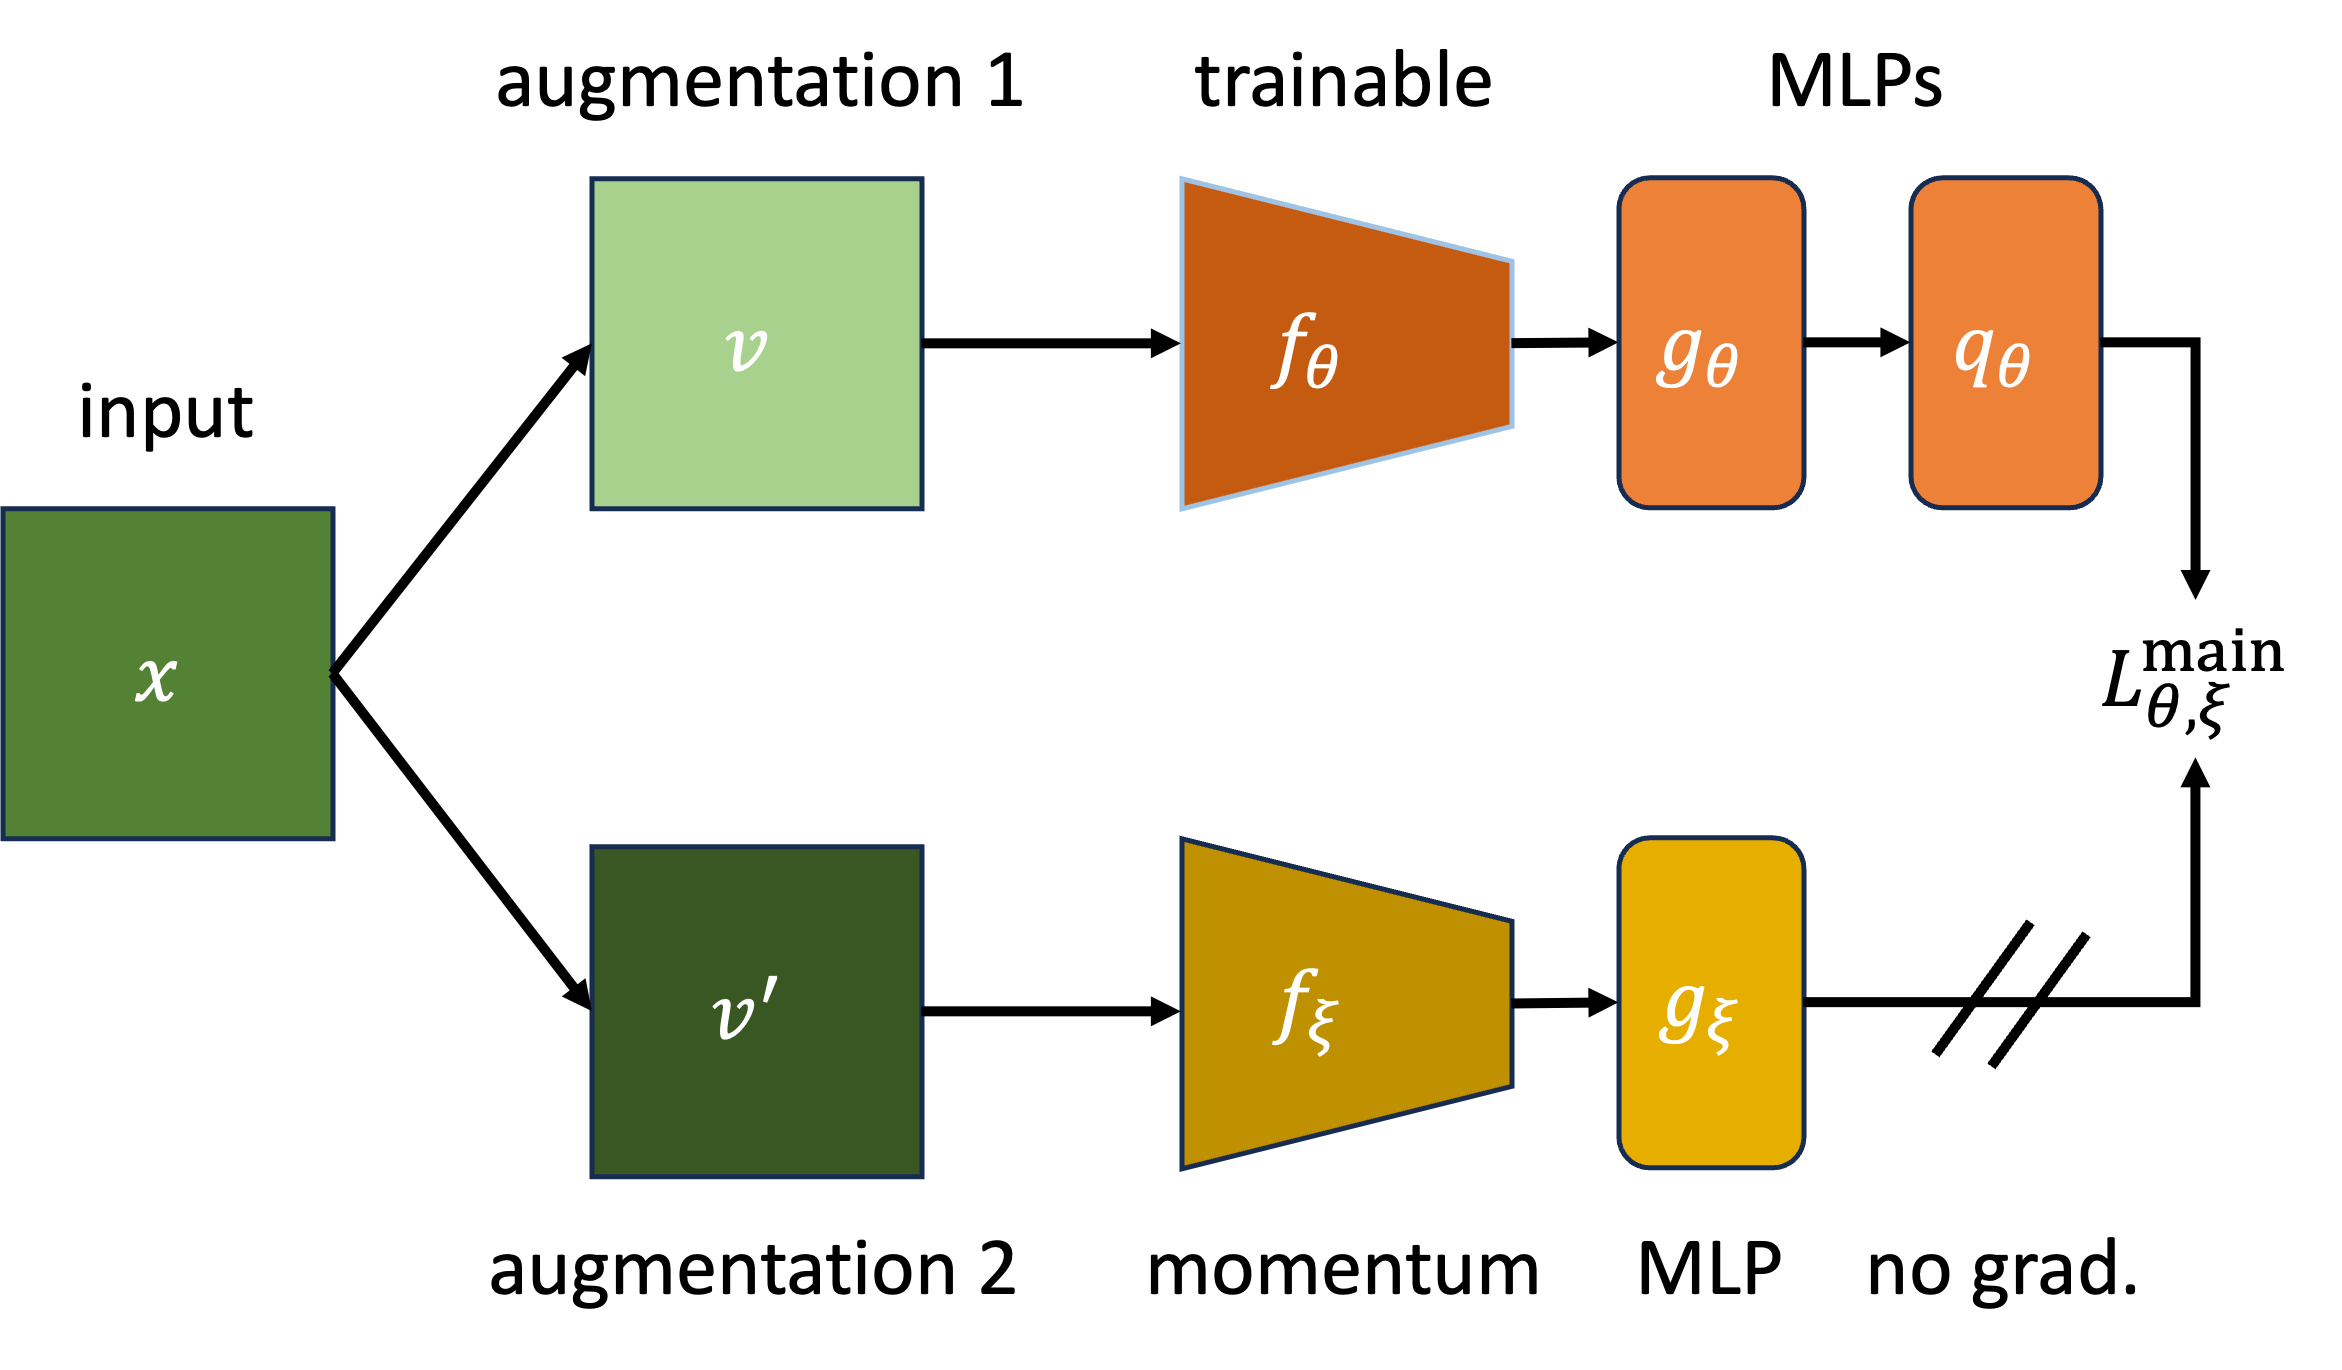
\includegraphics[width=\textwidth]{FIGURES/rlpl/rl1.png}
        \caption{main loss calculation}
        \label{fig:main loss}
    \end{subfigure}
    \hspace{0.02\textwidth} % Adjust space here
    % Second subfigure
    \begin{subfigure}[b]{0.45\textwidth}
        \centering
        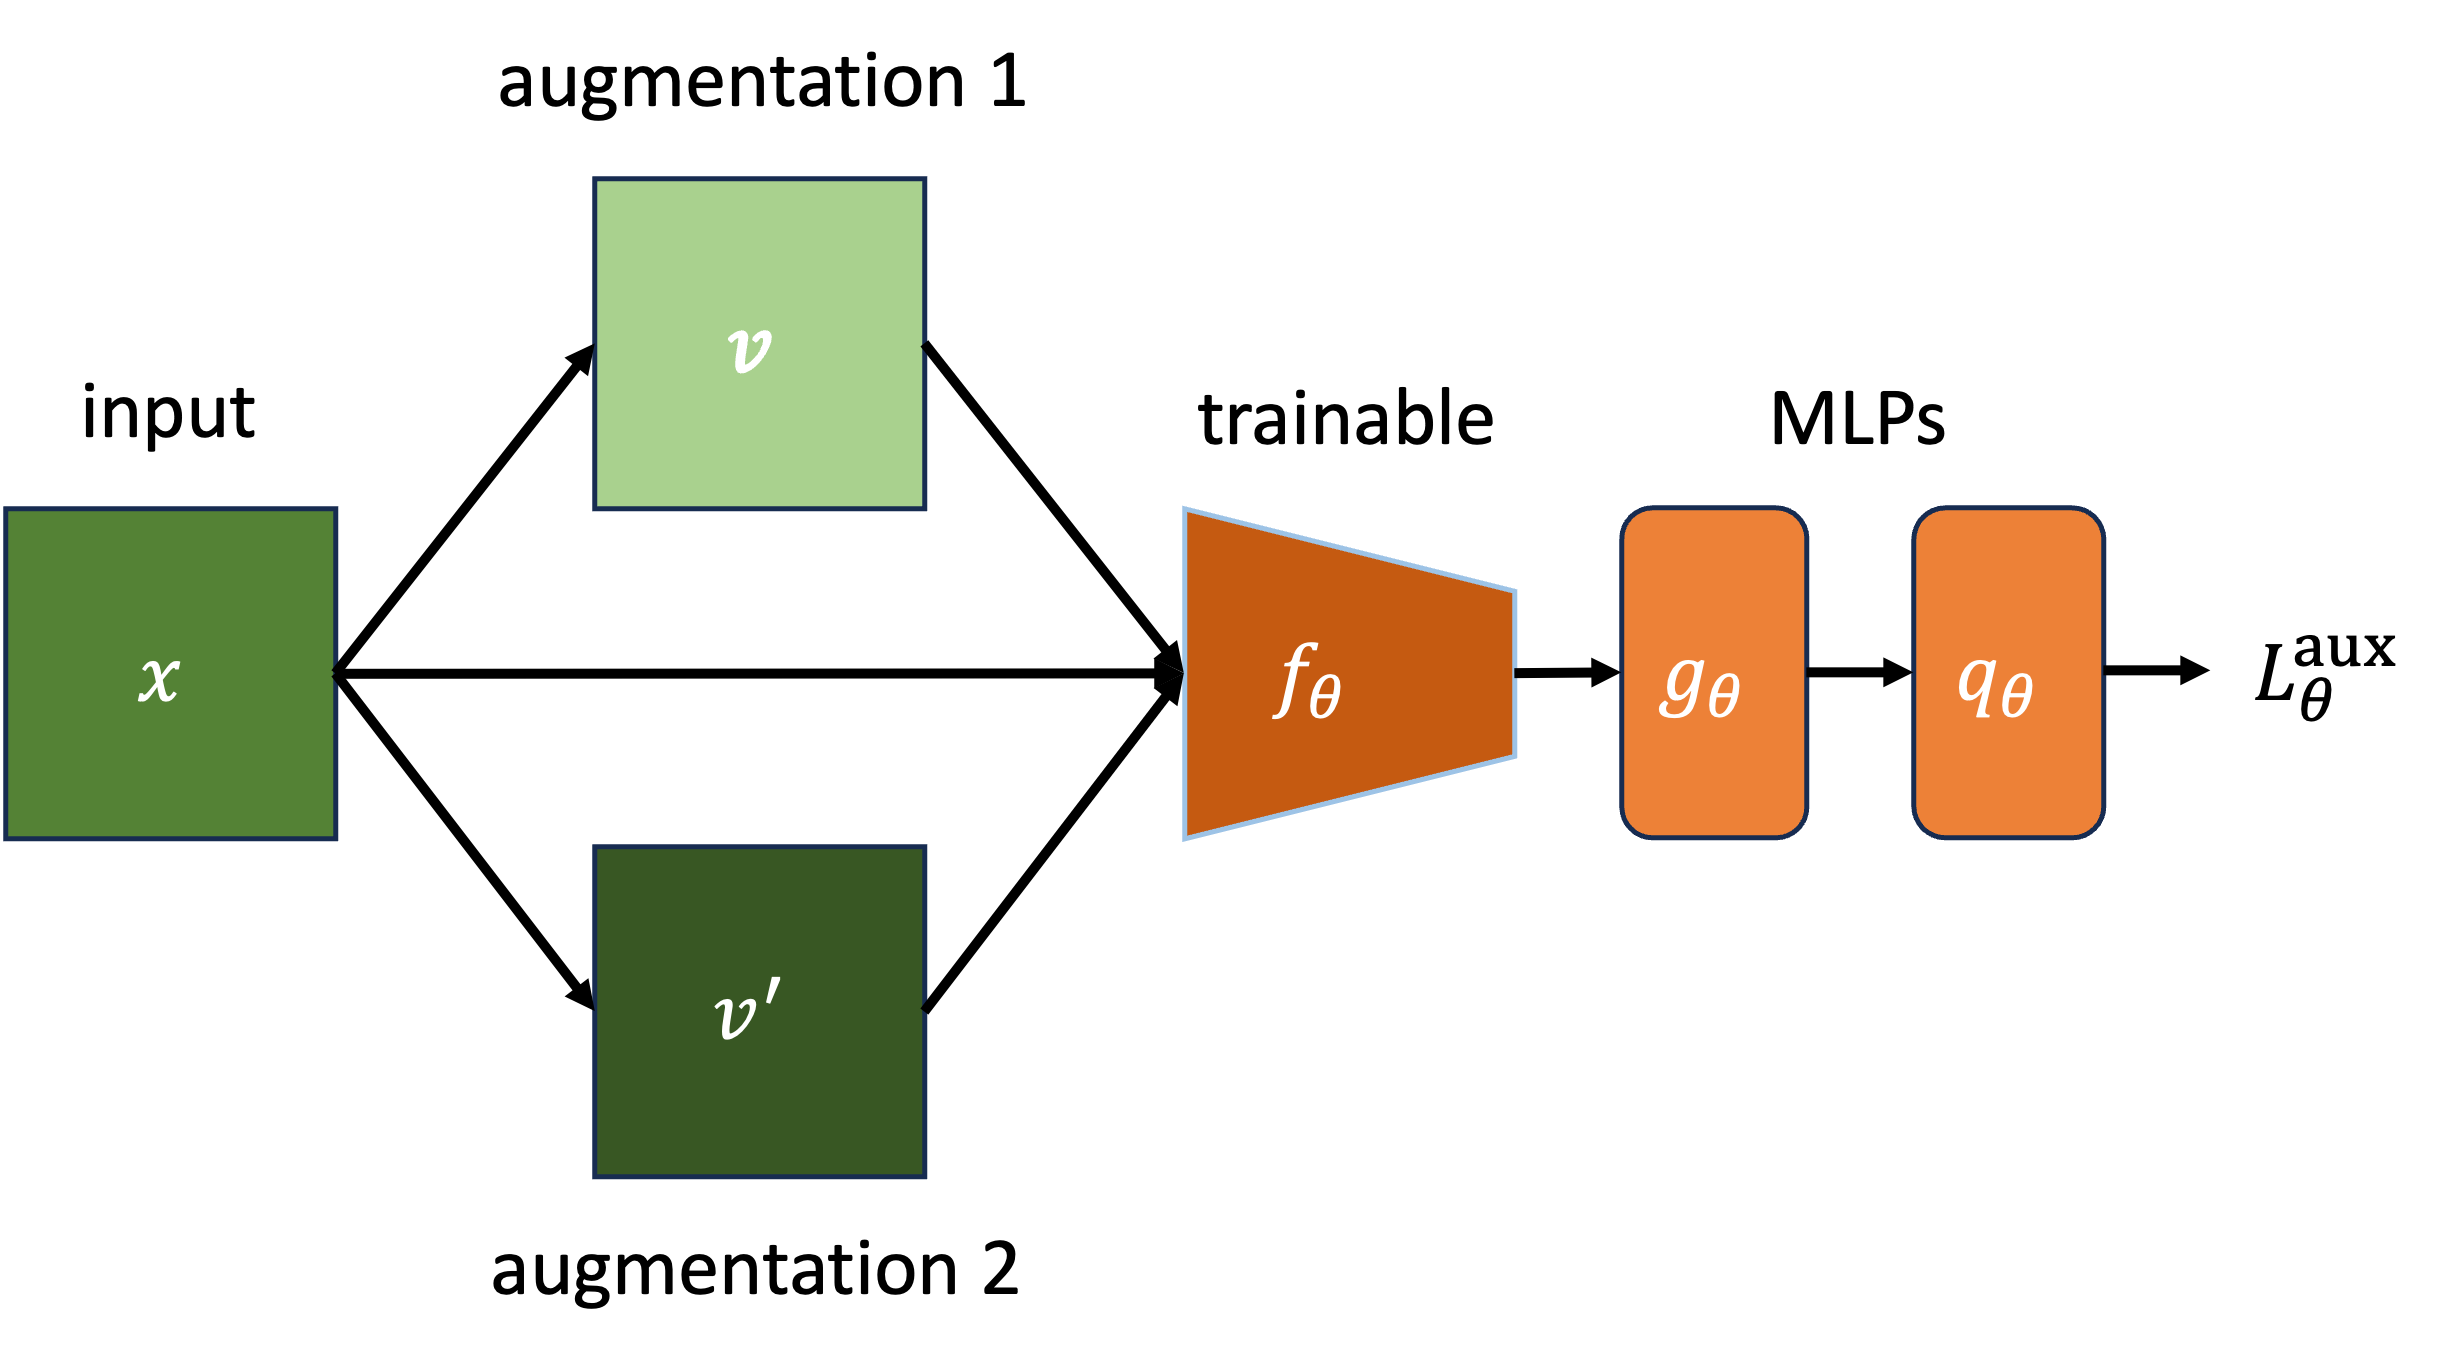
\includegraphics[width=\textwidth]{FIGURES/rlpl/rl2.png}
        \caption{auxiliary loss calculation}
        \label{fig:aux loss}
    \end{subfigure}
    
    \caption{Representation learning with RLPL: \textbf{(a)} The augmented inputs are processed through both networks to compute the main loss. \textbf{(b)} The original and augmented inputs are fed into the trainable network to compute the auxiliary loss.
    }

    \label{fig:two_photos}
\end{figure*}

RLPL learns a representation $y_{\theta}$ for downstream tasks using  encoder $f_{\theta}$, a projector $g_{\theta}$, and a predictor $q_{\theta}$. The momentum network, $f_{\xi}$, with a projector $g_{\xi}$, mirrors the trainable network's architecture but updates as an exponential moving average with decay rate, $\gamma \in [0,1]$:

\begin{equation}
\xi \leftarrow \gamma \xi + (1 - \gamma) \theta.
\end{equation}

For an input image $x$, we create two augmented views $v$ and ${v}'$. The trainable network computes $y_{\theta} \triangleq f_{\theta}(v)$ and $z_{\theta} \triangleq g_{\theta}(y_{\theta})$, while the momentum network outputs $y'_{\xi} \triangleq f_{\xi}(v')$ and $z'_{\xi} \triangleq g_{\xi}(y'_{\xi})$.

We then predict $z'_{\xi}$ from $z_{\theta}$ using $q_{\theta}(z_{\theta})$, and $l_2$-normalize both $q_{\theta}(z_{\theta})$ and $z'_{\xi}$ to $\bar{q}_{\theta}(z_{\theta}) \triangleq \frac{q_{\theta}(z_{\theta})}{\| q_{\theta}(z_{\theta}) \|_{2}}$ and $\bar{z}'_{\xi} \triangleq \frac{z'_{\xi}}{\| z'_{\xi} \|_{2}}$. The loss function is the mean squared error between the normalized prediction and momentum projection (as shown in Figure \ref{fig:main loss}):

\begin{equation} \label{eq:loss}
L_{\theta, \xi} \triangleq \left\| \bar{q}_{\theta}(z_{\theta}) - \bar{z}'_{\xi} \right\|_{2}^{2} = 2 - 2 \cdot \frac{\langle q_{\theta}(z_{\theta}), z'_{\xi} \rangle}{\| q_{\theta}(z_{\theta}) \|_{2} \cdot \| z'_{\xi} \|_{2}}.
\end{equation}

To symmetrize the loss, we feed $v'$ to the trainable network and $v$ to the momentum network, computing $\tilde{L}_{\theta, \xi}$. The combined loss for optimization is:

\begin{equation}
L_{\theta, \xi}^{\text{main}} = L_{\theta, \xi} + \tilde{L}_{\theta, \xi}.
\end{equation}

To calculate the auxiliary loss, the original image goes through the online network as an additional input (as shown in Figure \ref{fig:aux loss}). For original input $x$ and augmented views $v, v'$, we obtain outputs $q_{\theta}(z_{\theta }^{x})\triangleq q_{\theta}(g_{\theta}(f_{\theta}(x)))$, $q_{\theta}(z_{\theta }^{v})\triangleq q_{\theta}(g_{\theta}(f_{\theta}(v)))$, and $q_{\theta}(z_{\theta }^{v'})\triangleq q_{\theta}(g_{\theta}(f_{\theta}(v')))$, respectively. We design an auxiliary loss that allows gradient flow during backpropagation. This auxiliary loss is combined with the main loss, weighted by a factor \(\lambda\). The momentum network stays the same, but the trainable network affects its update parameters.

We calculate the mean of two output embeddings, $\bar{q_{\theta}}(z_{\theta }^{vv'})$, from the prediction head.

\begin{equation}
\bar{q_{\theta}}(z_{\theta }^{vv'}) =  \frac{1}{2}\left ( \bar{q_{\theta}}(z_{\theta}^{v}) + \bar{q_{\theta}}(z_{\theta}^{v'}) \right )
\end{equation}
where $\bar{q_{\theta}}(z_{\theta}^{v})$ and $\bar{q_{\theta}}(z_{\theta}^{v'})$ are the batch-mean of their respective embeddings, $q_{\theta}(z_{\theta}^{v})$ and $q_{\theta}(z_{\theta}^{v'})$.

Now, we denote the auxiliary loss as $L_{\theta}^{\text{aux}}$ and it is expressed as,
\begin{equation}
L_{\theta}^{\text{aux}} = \left \| \bar{q_{\theta}}(z_{\theta}^{x}) - \bar{q_{\theta}}(z_{\theta}^{vv'})\right \|_{2}^{2}
\end{equation}

where $\bar{q_{\theta}}(z_{\theta}^{x})$ is the batch-mean of ${q_{\theta}}(z_{\theta}^{x})$.

% \begin{equation}
% \text{mean}(\bar{q_{\Theta}^{v}}(z_{\Theta}), \bar{q_{\Theta}^{v'}}(z_{\Theta})) = \frac{\bar{q_{\Theta}^{v}}(z_{\Theta}) + \bar{q_{\Theta}^{v'}}(z_{\Theta})}{2}.
% \end{equation}

Next, it is added to the main loss with a weight, $\lambda$, to obtain the total loss.

\begin{equation}
L_{\theta, \xi} = L_{\theta, \xi}^{\text{main}} + \lambda L_{\theta}^{\text{aux}}
\end{equation}

% \noindent where $\lambda$ is the weight for the auxiliary loss.

Optimization updates the trainable network parameters $\theta$ with a learning rate $\eta$, while the momentum network parameters are updated as follows:

\begin{equation}
\theta \leftarrow \text{optimizer}(\theta, \nabla_{\theta} L_{\theta, \xi}, \eta),
\end{equation}

\begin{equation}
\xi \leftarrow \gamma \xi + (1 - \gamma) \theta.
\end{equation}

After training, only the encoder $f_{\theta}$ is returned for the downstream tasks. The pseudo-code for these steps is provided in Algorithm \ref{alg:bywl}.

% \begin{figure}[t]
\begin{algorithm}[!htbp]
\caption{Representation learning with RLPL} \label{alg:bywl}
\begin{algorithmic}
\State \textcolor{pythoncomment}{\# f\_t: trainable net (backbone + projector + predictor)}
\State \textcolor{pythoncomment}{\# f\_m: momentum net (backbone + projector)}
\State \textcolor{pythoncomment}{\# lambda: weight of auxiliary loss}
\State \textcolor{pythoncomment}{\# gma: momentum update rate}

\State \text{}
\State  \textcolor{pythonfunction}{for} x \textcolor{pythonfunction}{in} loader: \textcolor{pythoncomment}{\# load a minibatch}
\State \hspace{1.1em} v1, v2 = augment(x) \textcolor{pythoncomment}{\# two random augmentations}

\State \text{}

\State \hspace{1.1em} \textcolor{pythoncomment}{\# compute embeddings}
\State \hspace{1.1em}	t, t1, t2 = f\_t(x), f\_t(v1), f\_t(v2)  , \textcolor{pythoncomment}{\# $N \times D$}

\State \text{}

\State \hspace{1.1em}	\textcolor{purpleish}{with} torch.no\_grad(): \textcolor{pythoncomment}{\# stop the gradient}
\State \hspace{2.5em}	m1, m2 = f\_m(v1), f\_m(v2) \textcolor{pythoncomment} {\# $N \times D$}

\State \text{}

\State \hspace{1.1em} \textcolor{pythoncomment}{\# calculate the losses}
\State \hspace{1.1em}	loss\_main = (loss1(t1, m2) + loss1(t2, m1)).mean()
\State \hspace{1.1em} loss\_aux = loss2(t, t1, t2)
\State \hspace{1.1em}	total\_loss = loss\_main + lambda * loss\_aux
\State \hspace{1.1em} total\_loss.backward() \textcolor{pythoncomment}{\# optimization step}
\State \hspace{1.1em} update(f\_t.params)

\State \text{}

\State \hspace{1.1em} \textcolor{pythoncomment}{\# momentum network update}
\State \hspace{1.1em} f\_m.params = gma*f\_m.params+(1-gma)*f\_t.params

\State \text{}

\State \textcolor{pythonfunction}{def} loss1(a, b):  \textcolor{pythoncomment}{\# main loss function}
\State \hspace{1.1em} a = normalize(a, dim=-1)
\State \hspace{1.1em} b = normalize(b, dim=-1)
\State \hspace{1.1em} loss = 2 - 2 * (a * b).\textcolor{pythonfunction}{sum}(dim=-1) 
\State \hspace{1.1em} \textcolor{pythonfunction}{return} loss.mean()

\State \text{}

\State \textcolor{pythonfunction}{def} loss2(a, b, c): \textcolor{pythoncomment}{\# auxiliary loss function}
\State \hspace{1.1em}	avr\_emb = mean(b, c, dim=-1)
\State \hspace{1.1em} loss = loss1(a - avr\_emb)
\State \hspace{1.1em} \textcolor{pythonfunction}{return} loss.mean()
\end{algorithmic}
\end{algorithm}
% \end{figure}

\subsubsection{Effective Pseudo Labeling}  

For effective pseudo-labeling, let, $f_{\theta_T}$ and $f_{\theta_S}$ denote teacher and student networks initialized with parameters $\theta_T, \theta_S \leftarrow \theta$ from the pretrained encoder. Given a batch of labeled samples $(x_l, y_l) \in \mathcal{D}_l$ and unlabeled samples $x_u \in \mathcal{D}_u$, we formulate an iterative pseudo-labeling framework.

For each iteration, we first compute the student's initial loss on labeled data:

\begin{equation}
L_{s1} = \mathbb{E}_{(x_l,y_l)\sim\mathcal{D}_l}[\text{CE}(f_{\theta_S}(x_l), y_l)]
\end{equation}

For unlabeled data $x_u$, the teacher network generates soft pseudo-labels through weak augmentation $\mathcal{A}$:

\begin{equation}
\hat{y}_u = f_{\theta_T}(\mathcal{A}(x_u))
\end{equation}

To ensure quality of pseudo-labels, we filter predictions based on confidence threshold $\tau$:

\begin{equation}
\mathcal{M}_u = \{(x_u, \hat{y}_u) | \max(f_{\theta_T}(\mathcal{A}(x_u))) \geq \tau\}
\end{equation}

The teacher then learns from the filtered pseudo-labeled data:

\begin{equation}
L_u = \mathbb{E}_{(x_u,\hat{y}_u)\sim\mathcal{M}_u}[\text{CE}(f_{\theta_T}(x_u), \hat{y}_u)]
\end{equation}

After updating the student parameters using $L_u$, we measure its new performance:

\begin{equation}
L_{s2} = \mathbb{E}_{(x_l,y_l)\sim\mathcal{D}_l}[\text{CE}(f_{\theta_S}(x_l), y_l)]
\end{equation}

The effectiveness of pseudo-labeling is captured by the performance change:

\begin{equation}
\Delta L_s = L_{s2} - L_{s1}
\end{equation}

We incorporate this feedback through a meta-loss:

\begin{equation}
L_{\text{meta}} = \Delta L_s \cdot L_u
\end{equation}

The final objective for updating the teacher combines supervised learning on labeled data with the meta-loss feedback:

\begin{equation}
L_{\text{total}} = \underbrace{\mathbb{E}_{(x_l,y_l)\sim\mathcal{D}_l}[\text{CE}(f_{\theta_T}(x_l), y_l)]}_{\text{supervised loss}} + \underbrace{L_{\text{meta}}}_{\text{feedback}}
\end{equation}

This formulation creates a feedback loop where the teacher's pseudo-labeling strategy is dynamically adjusted based on the student's learning outcomes. When $\Delta L_s < 0$, indicating improved student performance, the teacher is encouraged to maintain its current strategy. Conversely, when $\Delta L_s > 0$, suggesting degraded performance, the teacher receives a stronger gradient signal to modify its approach.

The optimization proceeds iteratively:

\begin{align}
\theta_S &\leftarrow \theta_S - \eta_S \nabla_{\theta_S} L_u \\
\theta_T &\leftarrow \theta_T - \eta_T \nabla_{\theta_T} L_{\text{total}}
\end{align}

where $\eta_S$ and $\eta_T$ are learning rates for student and teacher networks respectively. After training convergence, only the teacher network is retained for deployment. The pseudo-code is provided in Algorithm~\ref{alg:PL}.

\begin{algorithm}[!htbp]
\caption{Pseudo labeling with RLPL} \label{alg:PL}
\begin{algorithmic}

\State \textcolor{pythoncomment}{\# f\_t: pretrained encoder}
\State \textcolor{pythoncomment}{\# n\_t, n\_s: teacher and student networks}
\State \textcolor{pythoncomment}{\# tau: pseudo labels threshold}

\State \text{}

% \State \textcolor{pythoncomment}{\# initialize teacher and student networks}

\State n\_t = f\_t.state\_dict() \textcolor{pythoncomment}{\# initialize teacher}
\State n\_s = f\_t.state\_dict() \textcolor{pythoncomment}{\# initialize student}

\State \text{}

\State \textcolor{pythoncomment}{\# load a minibatch of labeled and unlabeled samples}
\State  \textcolor{pythonfunction}{for} x, y, x\_u \textcolor{pythonfunction}{in} loader:
\State \hspace{1.1em}	\textcolor{purpleish}{with} torch.no\_grad(): \textcolor{pythoncomment}{\# stop the gradient}
\State \hspace{2.5em} loss\_s1 = cross\_entropy(n\_s(x), y)
\State \hspace{1.1em} y\_u = n\_t(x\_u) 

\State \text{}

\State \hspace{1.1em} \textcolor{pythoncomment}{\# filtering unlabled samples based on threshold}
\State \hspace{1.1em} x\_u, y\_u = x\_u $\left[  \text{y\_u} \geq \text{tau}\right]$, y\_u $\left[  \text{y\_u} \geq \text{tau}\right]$
\State \hspace{1.1em} y\_ut = n\_t(augment(x\_u))  \textcolor{pythoncomment}{\# weak augmentation}
\State \hspace{1.1em} loss\_t = cross\_entropy(y\_ut, y\_u)
\State \hspace{1.1em} loss\_t.backward()
\State \hspace{1.1em} update(n\_s.params) \textcolor{pythoncomment}{\# student network update}

\State \text{}

\State \hspace{1.1em}	\textcolor{purpleish}{with} torch.no\_grad(): \textcolor{pythoncomment}{\# stop the gradient}
\State \hspace{2.5em} loss\_s2 = cross\_entropy(n\_s(x), y)
\State \hspace{1.1em} change = loss\_s2 - loss\_s1
\State \hspace{1.1em} meta\_loss = change * loss\_t \textcolor{pythoncomment}{\# meta-loss computation}
\State \hspace{1.1em} loss = cross\_entropy(n\_t(x), y)
\State \hspace{1.1em} total\_loss = loss + meta\_loss \textcolor{pythoncomment}{\# total loss}
\State \hspace{1.1em} total\_loss.backward()
\State \hspace{1.1em} update(n\_t.params) \textcolor{pythoncomment}{\# teacher network update}

\end{algorithmic}
\end{algorithm}

\subsection{Experiments}

We conduct extensive experiments to evaluate RLPL's performance across multiple datasets and settings. Our analysis focuses on three key aspects: (1) the effect of batch size on representation learning quality, (2) comparison with state-of-the-art methods on standard benchmarks, and (3) ablation studies to validate our design choices. The following sections detail our experimental setup and findings.

\subsubsection{Datasets}

% In our experiments, we applied STL-10 \cite{singh2019justification}, CIFAR-10 \cite{ho2018cifar10} and SVHN \cite{sermanet2012convolutional} datasets for unlabeled RL training. The STL-10 dataset is specially designed for unsupervised feature learning as it contains $13,000$ labeled images across $10$ classes and $100,000$ unlabeled images. While we used the entire training set of CIFAR-10 and SVHN datasets for RL, we only used $250$, $1,000$, and $4,000$ labeled training samples in downstream classifications. Additional experiments were conducted on 6 other image datasets \cite{krizhevsky2009learning, xiao2017fashionmnist, LFWTech, helber2019eurosat, nilsback2008automated, imagenette2019} with different class numbers.

Our experiments utilized a diverse collection of image datasets to thoroughly evaluate the effectiveness of our proposed approach. Below, we provide a detailed description of each dataset used in our study:

\noindent \textbf{STL-10} \cite{singh2019justification} is specifically designed for unsupervised and self-supervised learning research. It contains 13,000 labeled images across 10 object categories (airplane, bird, car, cat, deer, dog, horse, monkey, ship, and truck) and 100,000 unlabeled images sampled from a similar but broader distribution. A key characteristic of STL-10 is its relatively high-resolution images (96×96 pixels), making it more challenging than lower-resolution alternatives. The limited labeled training set (500 images per class) combined with abundant unlabeled data makes it an ideal benchmark for semi-supervised learning approaches, closely mirroring real-world scenarios where labeled data is scarce.

\noindent \textbf{CIFAR-10} \cite{ho2018cifar10} consists of 60,000 color images (32×32 pixels) divided into 10 mutually exclusive classes (airplane, automobile, bird, cat, deer, dog, frog, horse, ship, truck). The dataset is split into 50,000 training and 10,000 test images, with each class having an equal number of samples. While the entire training set was used for representation learning, we specifically created label-limited scenarios with only 250, 1,000, and 4,000 labeled examples to evaluate model performance under varying degrees of supervision. This approach allows us to assess how effectively our method leverages unlabeled data when labeled samples are extremely scarce.

\noindent \textbf{SVHN} \cite{sermanet2012convolutional} (Street View House Numbers) is derived from Google Street View images and presents a real-world object recognition task focused on digit classification. It contains over 600,000 digit images in its complete version, with 73,257 digits for training, 26,032 for testing, and an additional 531,131 less difficult samples that can be used as extra training data. Unlike handwritten digit datasets, SVHN presents additional challenges with real-world variations in lighting, orientation, and background clutter. The images are 32×32 pixels in color, and like CIFAR-10, we constructed supervision-limited scenarios with 250, 1,000, and 4,000 labeled examples.

For transfer learning evaluation, we employed six additional image datasets with varying characteristics:

\noindent \textbf{CIFAR-100} \cite{krizhevsky2009learning} is similar to CIFAR-10 in image size (32×32 pixels) but contains 100 fine-grained classes grouped into 20 superclasses. With 600 images per class (500 training, 100 testing), it presents a more challenging fine-grained classification task.

\noindent \textbf{Fashion-MNIST} \cite{xiao2017fashionmnist} is designed as a more challenging drop-in replacement for the traditional MNIST dataset. It consists of 70,000 grayscale images (28×28 pixels) of fashion items across 10 categories, divided into 60,000 training and 10,000 test examples. This dataset helps evaluate model performance on grayscale images with more complex patterns than digits.

\noindent \textbf{LFW} \cite{LFWTech} (Labeled Faces in the Wild) contains 13,233 face images of 5,749 individuals collected from the web. These images present natural variations in pose, lighting, expression, and background, making it a challenging benchmark for face recognition tasks. We used the aligned version of the dataset with cropped faces.

\noindent \textbf{EuroSAT} \cite{helber2019eurosat} is a land use and land cover classification dataset derived from Sentinel-2 satellite imagery. It contains 27,000 labeled images (64×64 pixels) across 10 classes, representing various land use patterns. This dataset helps evaluate the model's performance on remote sensing applications.

\noindent \textbf{Oxford Flowers 102} \cite{nilsback2008automated} includes 8,189 images of 102 flower categories common in the United Kingdom. Each class contains between 40-258 images with significant variations in scale, pose, and lighting. This fine-grained classification task presents a different challenge due to its natural image variability and smaller sample size per class.

\noindent \textbf{Imagenette} \cite{imagenette2019} is a subset of 10 easily distinguishable classes from ImageNet (tench, English springer, cassette player, chain saw, church, French horn, garbage truck, gas pump, golf ball, parachute). With approximately 13,000 training images and larger dimensions than the other datasets, it tests the model's ability to handle higher-resolution natural images.

This diverse collection of datasets enables a comprehensive evaluation of our proposed method across a wide range of image domains, resolutions, class numbers, and task difficulties, demonstrating its versatility and general applicability to various computer vision scenarios.


\subsubsection{Implementation Details} 

\textbf{Image augmentations:} Our augmentation pipeline follows SimCLR and BYOL, using PyTorch~\cite{paszke2019pytorch}. We apply "RandomResizedCrop" (scale: [0.2, 1.0]), "RandomHorizontalFlip", "ColorJitter" (brightness, contrast, saturation: 0.4, hue: 0.1), "RandomGrayscale" (p=0.2), and "GaussianBlur" ($\sigma$=[1.0, 2.0], p=0.2). Images are normalized using standard mean and variance values. 

Our experiments reveal that image resolution significantly affects accuracy; thus, we resize all images to \(256 \times 256\). In the PL phase, weak augmentations are applied to the teacher model, involving random horizontal and vertical flips, each with a probability of \(0.25\).

\noindent
\textbf{Architecture:} We use ResNet18 \cite{ayyachamy2019medical}, a more computationally feasible network, designed for GPU computations. This ResNet18 architecture remains consistent across all settings, including representation learning, and pseudo labeling. The MLPs, projection, and prediction layers adhere to the parameters established by BYOL. In PL, the teacher and student networks are initialized from the ResNet18, pre-trained via RL.

\noindent
\textbf{Optimization:} The RL framework was optimized using the Adam optimizer \cite{zhang2018improved}, whereas PL employed the Stochastic Gradient Descent (SGD) optimizer \cite{gower2019sgd}, both with a learning rate set to $0.0003$. The auxiliary loss is weighted at \(0.5\). RL underwent training for $50$ epochs with a batch size of $128$, while PL was trained over $150$ epochs with a batch size of $16$.

\begin{figure}[!htbp]
    \centering
    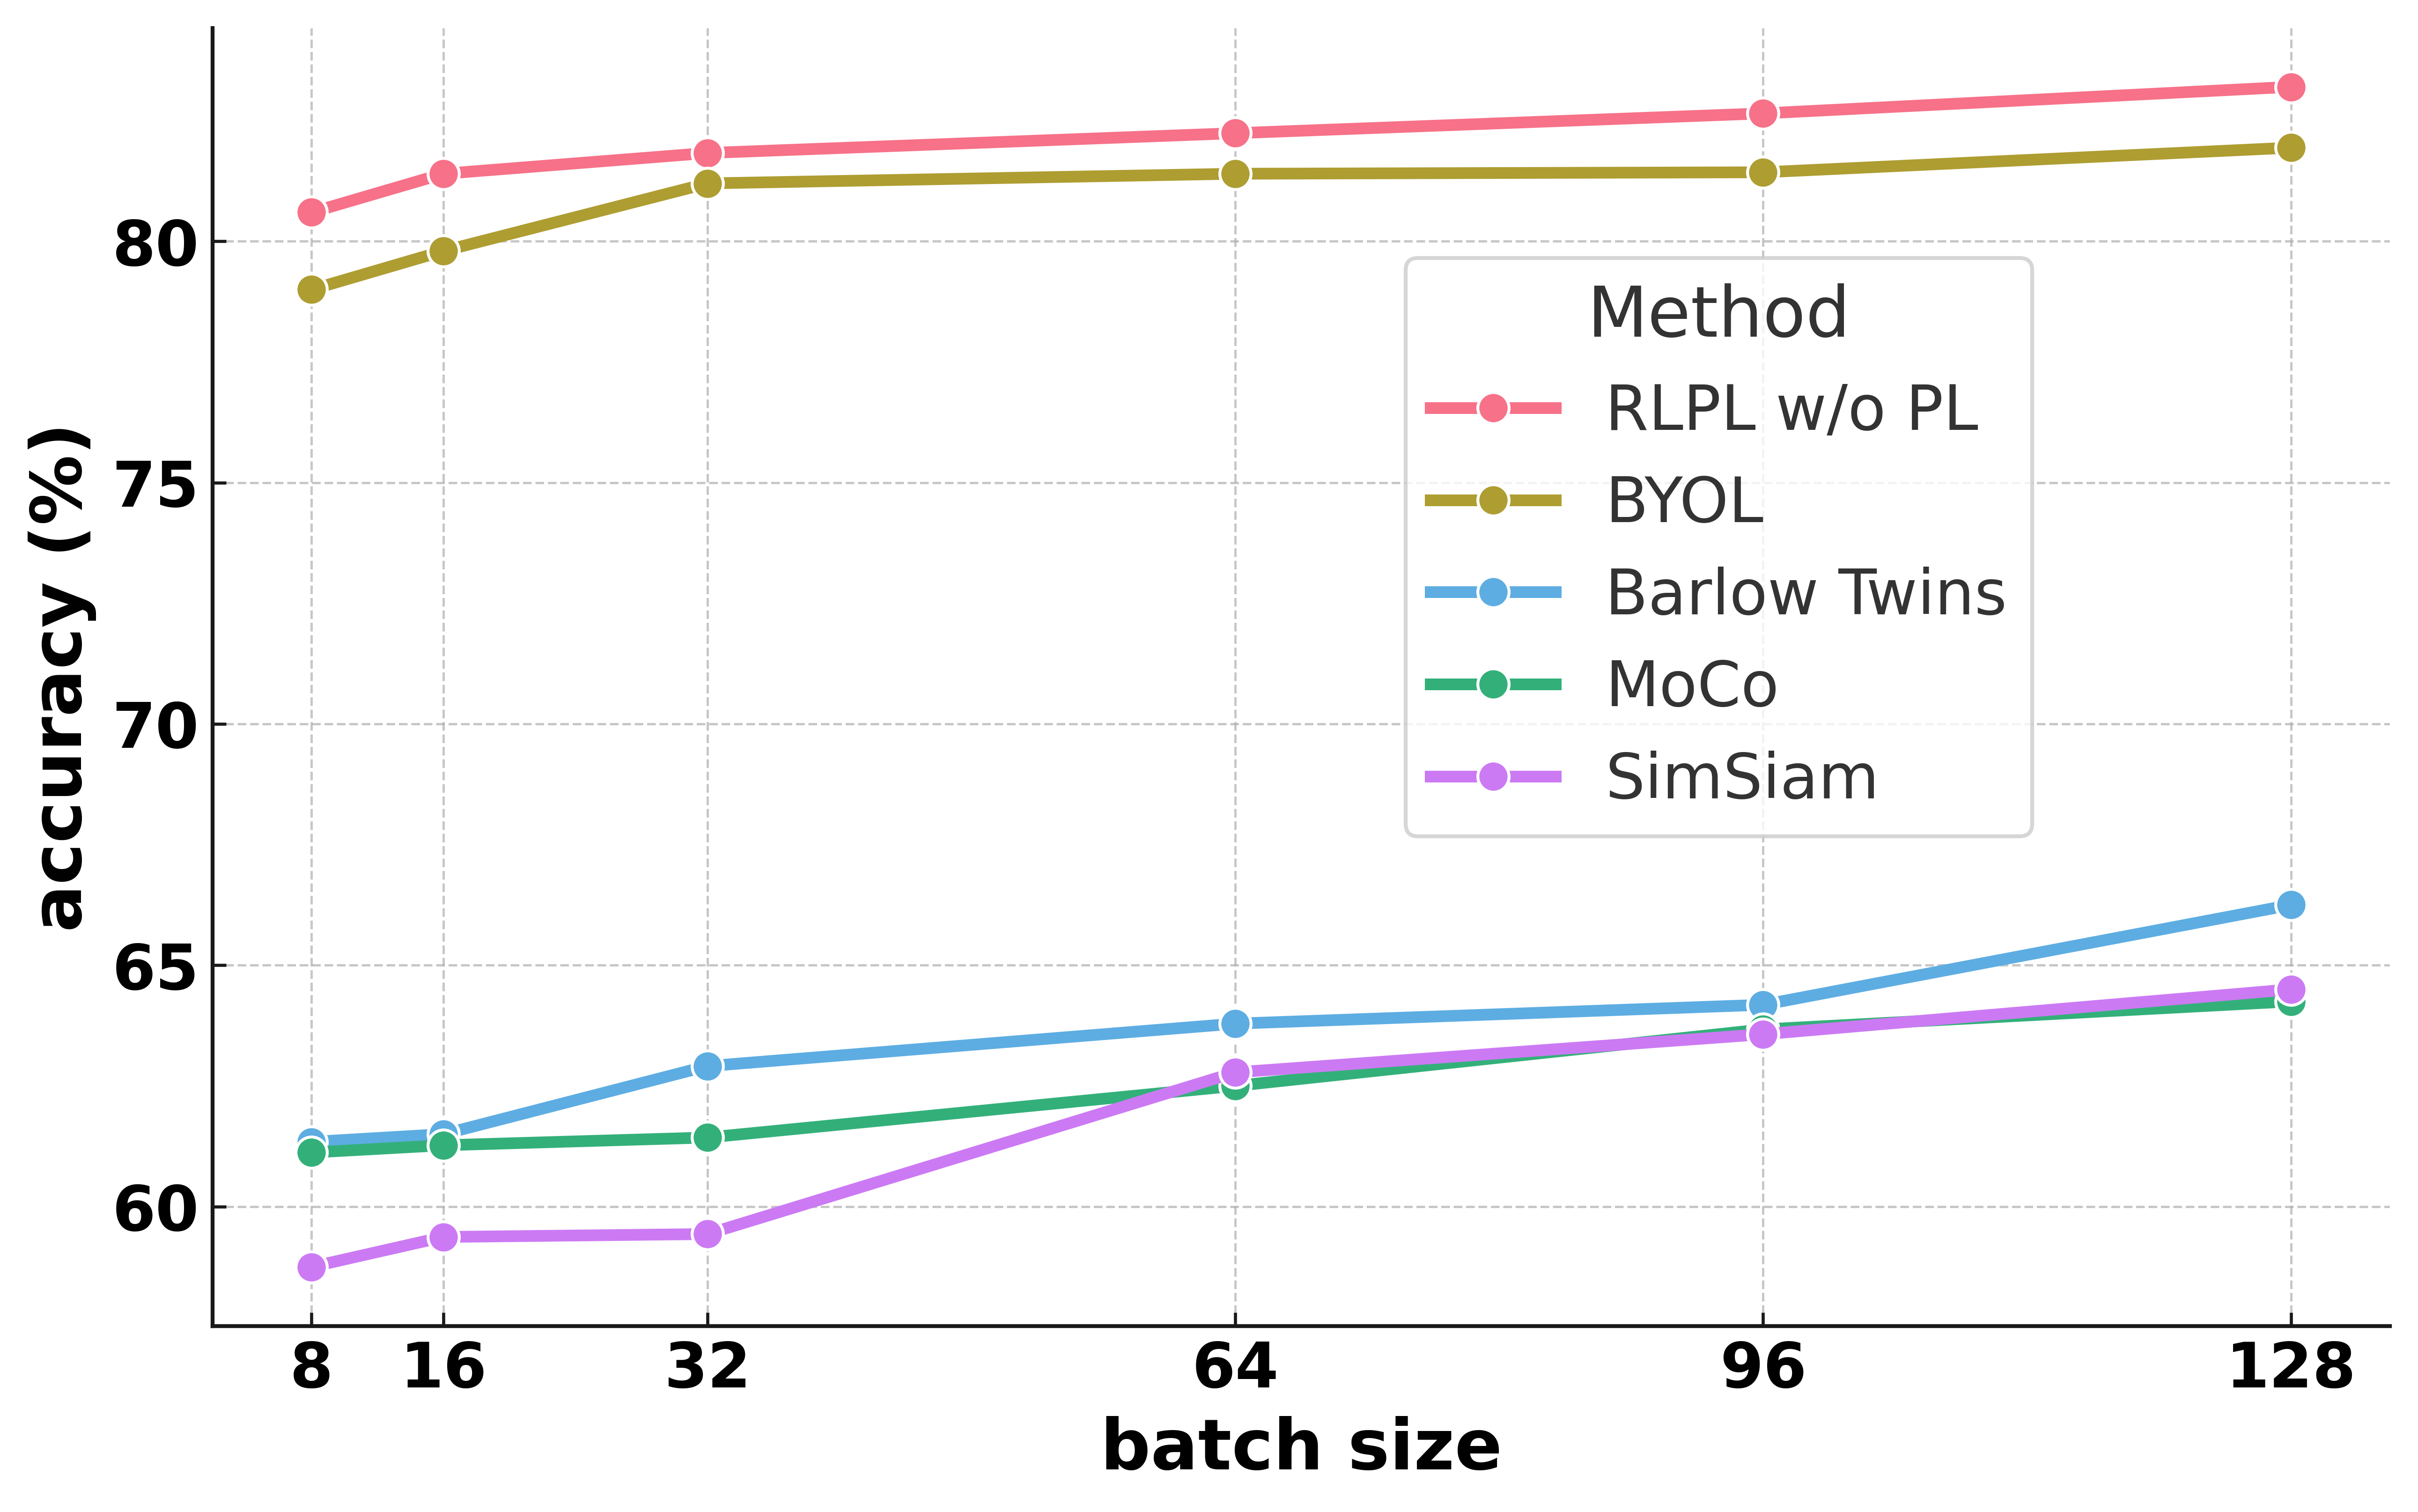
\includegraphics[width=0.9\columnwidth, keepaspectratio]{FIGURES/rlpl/accuracy_vs_batch.png}
    \caption{Effect of batch size on model performance (evaluated on STL-10).}
    \label{fig:batch}
\end{figure}

\begin{table}[htbp]
    \centering
    \begin{tabular}{l c}
      \toprule
      \textbf{Methods} & \textbf{Test Accuracy (\%)} \\  
      \midrule
      Baseline (ResNet18) & 53.16 \\
      FixMatch \cite{sohn2020fixmatch} & 37.28 \\ 
      MixMatch \cite{berthelot2019mixmatch} & 71.60 \\
      MoCo & 66.25 \\
      SimSiam & 64.50 \\
      Barlow Twins & 64.25 \\
      BYOL & 81.94  \\
      RLPL (Ours) & \textbf{84.64} \\
      \bottomrule
    \end{tabular}
    \caption{Performance of different methods on STL-10 dataset.}
    \label{table:stl}
\end{table}

\subsection{Results and Discussion}

\begin{table}[htbp]
    \centering
    \resizebox{\textwidth}{!}{%
    \begin{tabular}{llllllll}
    \hline
    \multirow{2}{*}{\bf Method} & \multicolumn{3}{c}{\bf CIFAR-10} & \multicolumn{3}{c}{\bf SVHN} & \multirow{2}{*}{\bf Average} \\ 
    \cmidrule(lr){2-4} \cmidrule(lr){5-7}
     & \bf 250 labels & \bf 1000 labels & \bf 4000 labels & \bf 250 labels & \bf 1000 labels & \bf 4000 labels & \\ \hline
    ResNet18 & 33.90 & 43.71 & 58.47 & 41.20 & 84.58 & 87.60 & 58.24 \\
    MoCO     & 34.50 & 46.75 & 61.88 & 30.75 & 83.25 & 89.12 & 57.37 \\
    SimSiam  & 23.88 & 29.50 & 48.88 & 14.62 & 51.25 & 67.38 & 39.92 \\
    Barlow Twins & 35.88 & 47.75 & 63.75 & 21.88 & 79.01 & 88.25 & 56.42 \\
    BYOL     & 33.19 & 46.92 & 59.29 & 67.00 & 85.60 & 88.20 & 63.70 \\
    RLPL (ours) & \bf 48.93 & \bf 52.45 & \bf 65.69 & \bf 72.12 & \bf 88.39 & \bf 92.78 & \bf 70.39 \\ \hline
    \end{tabular}%
    }
    \caption{Test accuracy (\%) of different methods on varying numbers of training samples.}
    \label{table:2}
\end{table}


\begin{table}[!htbp]
\centering
\resizebox{\textwidth}{!}{
\begin{tabular}{lllllllll}
\hline
\multirow{2}{*}{\bf Method} & \multirow{2}{*}{\bf STL-10} & \multicolumn{3}{c}{\bf CIFAR-10}           & \multicolumn{3}{c}{\bf SVHN} & \multirow{2}{*}{\bf Average} \\ \cmidrule(lr){3-5}\cmidrule(lr){6-8}
                 &       & \bf 250 labels & \bf 1000 labels & \bf 4000 labels & \bf 250 labels & \bf 1000 labels & \bf 4000 labels & \\ \hline
PL (random init.)      &     53.34         &    30.49        &     40.57        &   55.90         &        11.19    &      17.62       &    75.62       &   40.39 \\
RLPL w/o PL      &      83.20        &    34.54       &     48.48        &   59.60          &     71.25      &       85.54      &     89.00      &   67.66 \\
RLPL (ours)    &    \bf 84.64       & \bf  48.93        &   \bf     52.45     &  \bf     65.69      & \bf    72.12       &    \bf   88.39     &  \bf   92.78  & \bf 72.14 \\ \hline
\end{tabular}
}
\captionof{table}{Test accuracy (\%) for ablation on methods.}
\label{table:ablation}
\end{table}


Our evaluation methods primarily comprise the baseline model, BYOL, SimSiam, MoCo, Barlaw Twins, RLPL, and two additional semi-supervised algorithms, FixMatch \cite{sohn2020fixmatch}, and MixMatch \cite{berthelot2019mixmatch} on the considered datasets. In all our experiments, we re-implemented each algorithm on a ResNet18 backbone with identical hyperparameters to ensure a fair comparison.

\subsubsection{Effect of Batch Size}

To illustrate the effectiveness of RLPL with reduced batch sizes, we present the results in Figure \ref{fig:batch}. We started with a batch size of $8$ for RLPL. Subsequently, we gradually increased the batch sizes for RLPL and others to evaluate their performances. To have a fair comparison, we applied the classification tasks only on the learned representation of RL, without any use of PL. As anticipated, the accuracy diminished with smaller batch sizes. Remarkably, at a batch size of $64$, RLPL attained an accuracy of $82.24\%$, surpassing BYOL's accuracy of $81.94\%$ with a batch size of $128$. All other methods, including Barlow Twins, MoCo, and SimSiam, achieve significantly lower accuracy in the small-scale implementation, with their performance further declining as batch size decreases. Although all methods exhibited a decline in accuracy with further reductions in batch sizes, RLPL consistently outperformed BYOL and all the others.

\subsubsection{Classification Accuracy}

Table \ref{table:stl} reports the classification accuracy on the STL-10 dataset. The ResNet18 classifier demonstrates challenges in reaching acceptable accuracy levels. For a fair comparison, all methods, including FixMatch and MixMatch, were implemented with a ResNet18 backbone and an identical batch size.

The results reveal that FixMatch struggles to achieve competitive accuracy, likely due to the limitations of pseudo-labeling techniques, which often require robust initialization and a deep backbone to perform effectively. While MixMatch shows considerable improvement, it still falls short of the performance attained by BYOL and RLPL. MoCo, SimSiam, and Barlow Twins achieve almost similar but lower accuracy. Notably, BYOL achieves an accuracy of $81.94\%$, whereas RLPL surpasses this with an accuracy of $84.64\%$, obtaining a $\textbf{2.7\%}$ improvement over BYOL.

Table \ref{table:2} compares ResNet18, the four primary methods central to this study, and RLPL across varying training samples. For both datasets, all methods showed progressively higher accuracies with increasing sample sizes. We observe that our method uniquely achieves acceptable accuracy on CIFAR-10 with only 250 labels, whereas other methods struggle under the same conditions. For SVHN with 250 labels, only BYOL and RLPL reach satisfactory accuracy, while other methods perform notably worse. Notably, Notably, RLPL consistently achieved the highest accuracy across all datasets and under all varying configurations, outperforming other methods in each case.

We include a column displaying the average test accuracy across all setups to provide a comprehensive view of the relative performance of each method. Only BYOL comes close to RLPL's performance; however, it still lags by a margin of \textbf{6.69\%}. Nevertheless, RLPL consistently outperformed BYOL across all scenarios, particularly with smaller sample sizes, with improvement margins ranging from $\textbf{2.79\%}$ to $\textbf{15.74\%}$.

\subsubsection{Transfer to Other Classification Tasks}

\begin{table}[htbp]
    \centering
    \resizebox{\textwidth}{!}{%
    \begin{tabular}{lccccccc}
    \hline
    \textbf{Method} & \textbf{CIFAR100} & \textbf{FashionMNIST} & \textbf{LFW} & \textbf{EuroSAT} & \textbf{OxfordFlowers102} & \textbf{Imagenette} & \bf Average \\ \hline
    ResNet18 & 58.09 & 94.55 & 85.03 & 93.62 & 38.48 & 80.66 & 75.07 \\
    MoCo & 62.50 & 90.54 & \bf 93.21 & 95.00 & 35.00 & 79.88 & 76.69 \\
    SimSiam & 33.88 & 92.63 & 80.41 & 79.38 & 26.12 & 76.82 & 64.54 \\
    Barlow Twins & 58.75 & 94.38 & 89.19 & 94.62 & 27.88 & 80.38 & 74.87 \\
    BYOL & 63.61 & 93.62 & 80.73 & \bf 96.28 & 49.64 & 86.13 & 78.67 \\
    RLPL w/o PL & \bf 68.08 & \bf 96.01 & 89.33 & 96.03 & \bf 51.67 & \bf 87.94 & \bf 81.51 \\ \hline
    \end{tabular}%
    }
    \caption{Performance comparison (\% test accuracy) of methods on various datasets.}
    \label{table:transfer}
\end{table}

We evaluated RLPL's generalization on diverse classification tasks, as shown in Table~\ref{table:transfer}. This table compares RLPL's performance with baseline and other methods after pretraining on the STL-10 dataset, followed by the downstream tasks. For a fair comparison, we applied the pretrained RLPL model directly, without using PLs in the classification tasks. This approach highlights RLPL's standalone performance; notably, integrating PL strategies could likely enhance accuracy beyond the presented results.

RLPL achieves the highest accuracy in nearly all cases, except for MoCo on the Labeled Faces in the Wild (LFW) dataset and BYOL on the EuroSAT dataset. RLPL obtains an average accuracy of 81.51\%, substantially outperforming methods like SimSiam and Barlow Twins. Moreover, RLPL obtains $\textbf{2.84\%}$ more accuracy than the closest best method, BYOL, across all the transfer learning tasks. This improvement highlights RLPL's transferability on unseen classification tasks.

\subsection{Ablation Study}

To validate our design choices and understand the contribution of each component, we conducted comprehensive ablation studies. We analyzed the impact of representation learning, pseudo-labeling, and their combination across different datasets and label regimes. Additionally, we investigated the effects of key hyperparameters like auxiliary loss weight and pseudo-label thresholds.

\subsubsection{Framework Ablation}

\begin{figure}[htbp]
\centering
\begin{subfigure}[t]{0.45\textwidth}
    \centering
    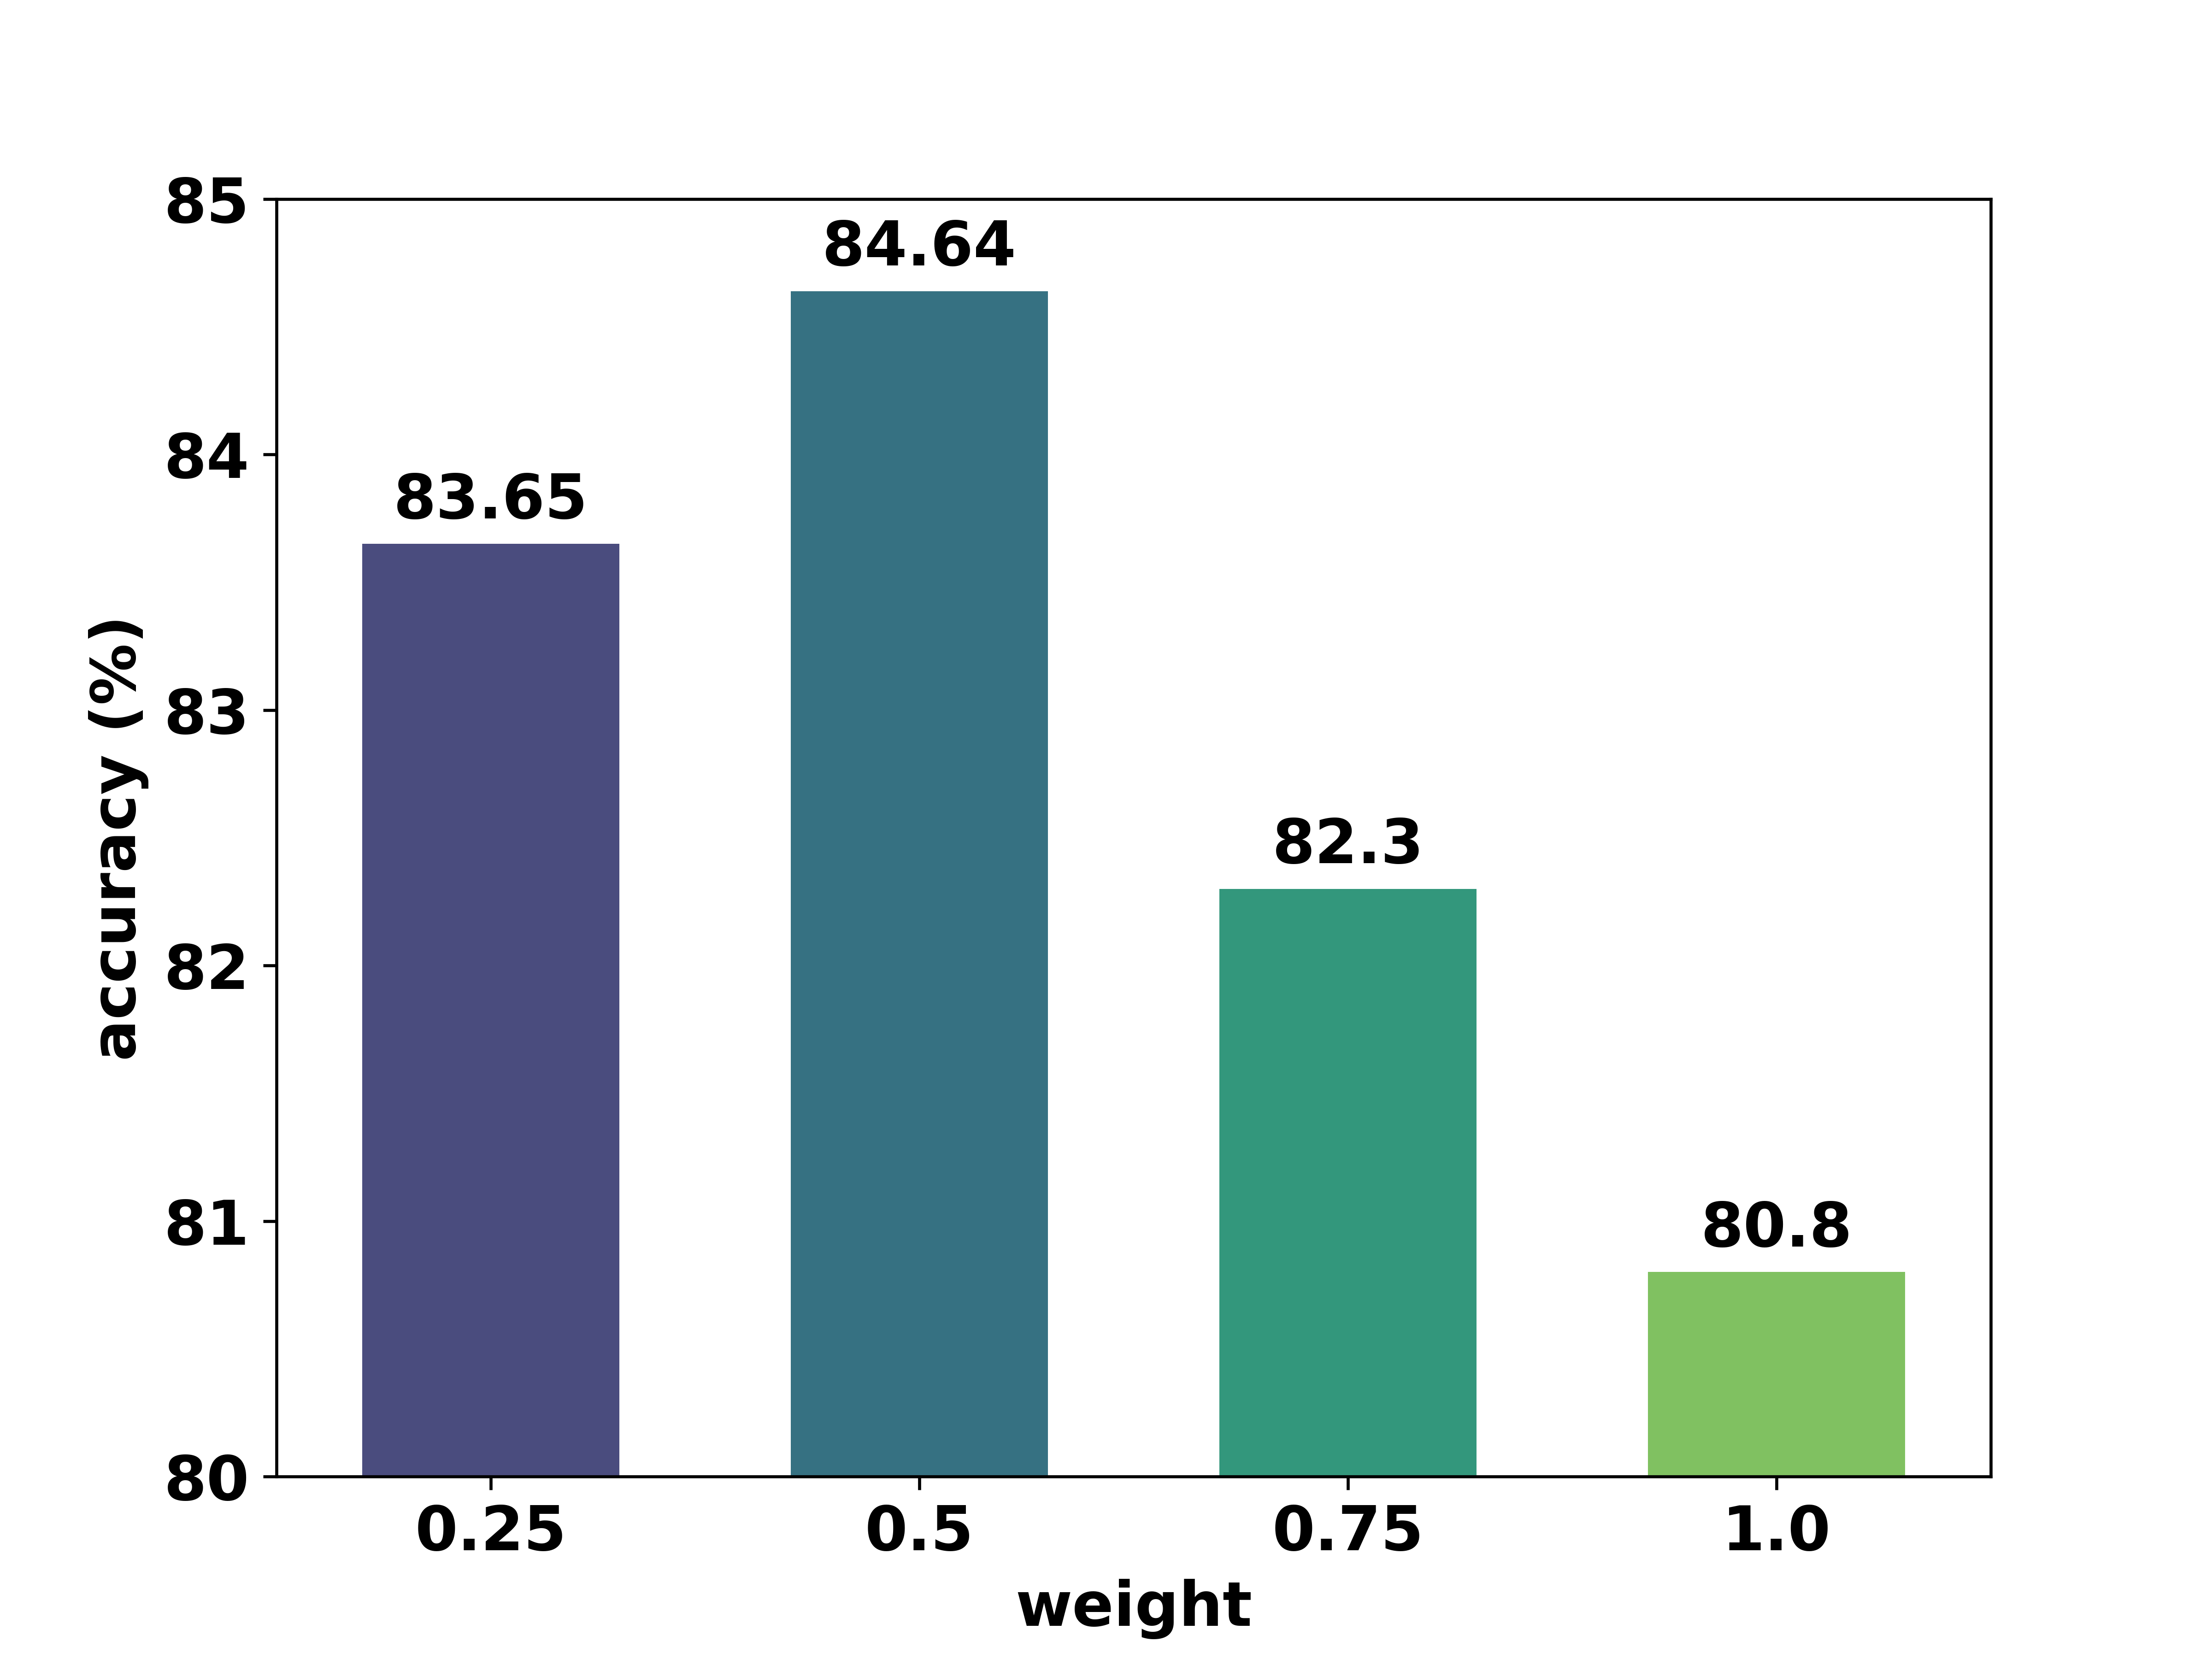
\includegraphics[width=\linewidth]{FIGURES/rlpl/accuracy_vs_weight.png}
    \caption{Effect of the auxiliary loss weight, $\lambda$.}
    \label{fig:weight}
\end{subfigure}%
\hspace{0.05\textwidth} % Adjust space here
\begin{subfigure}[t]{0.45\textwidth}
    \centering
    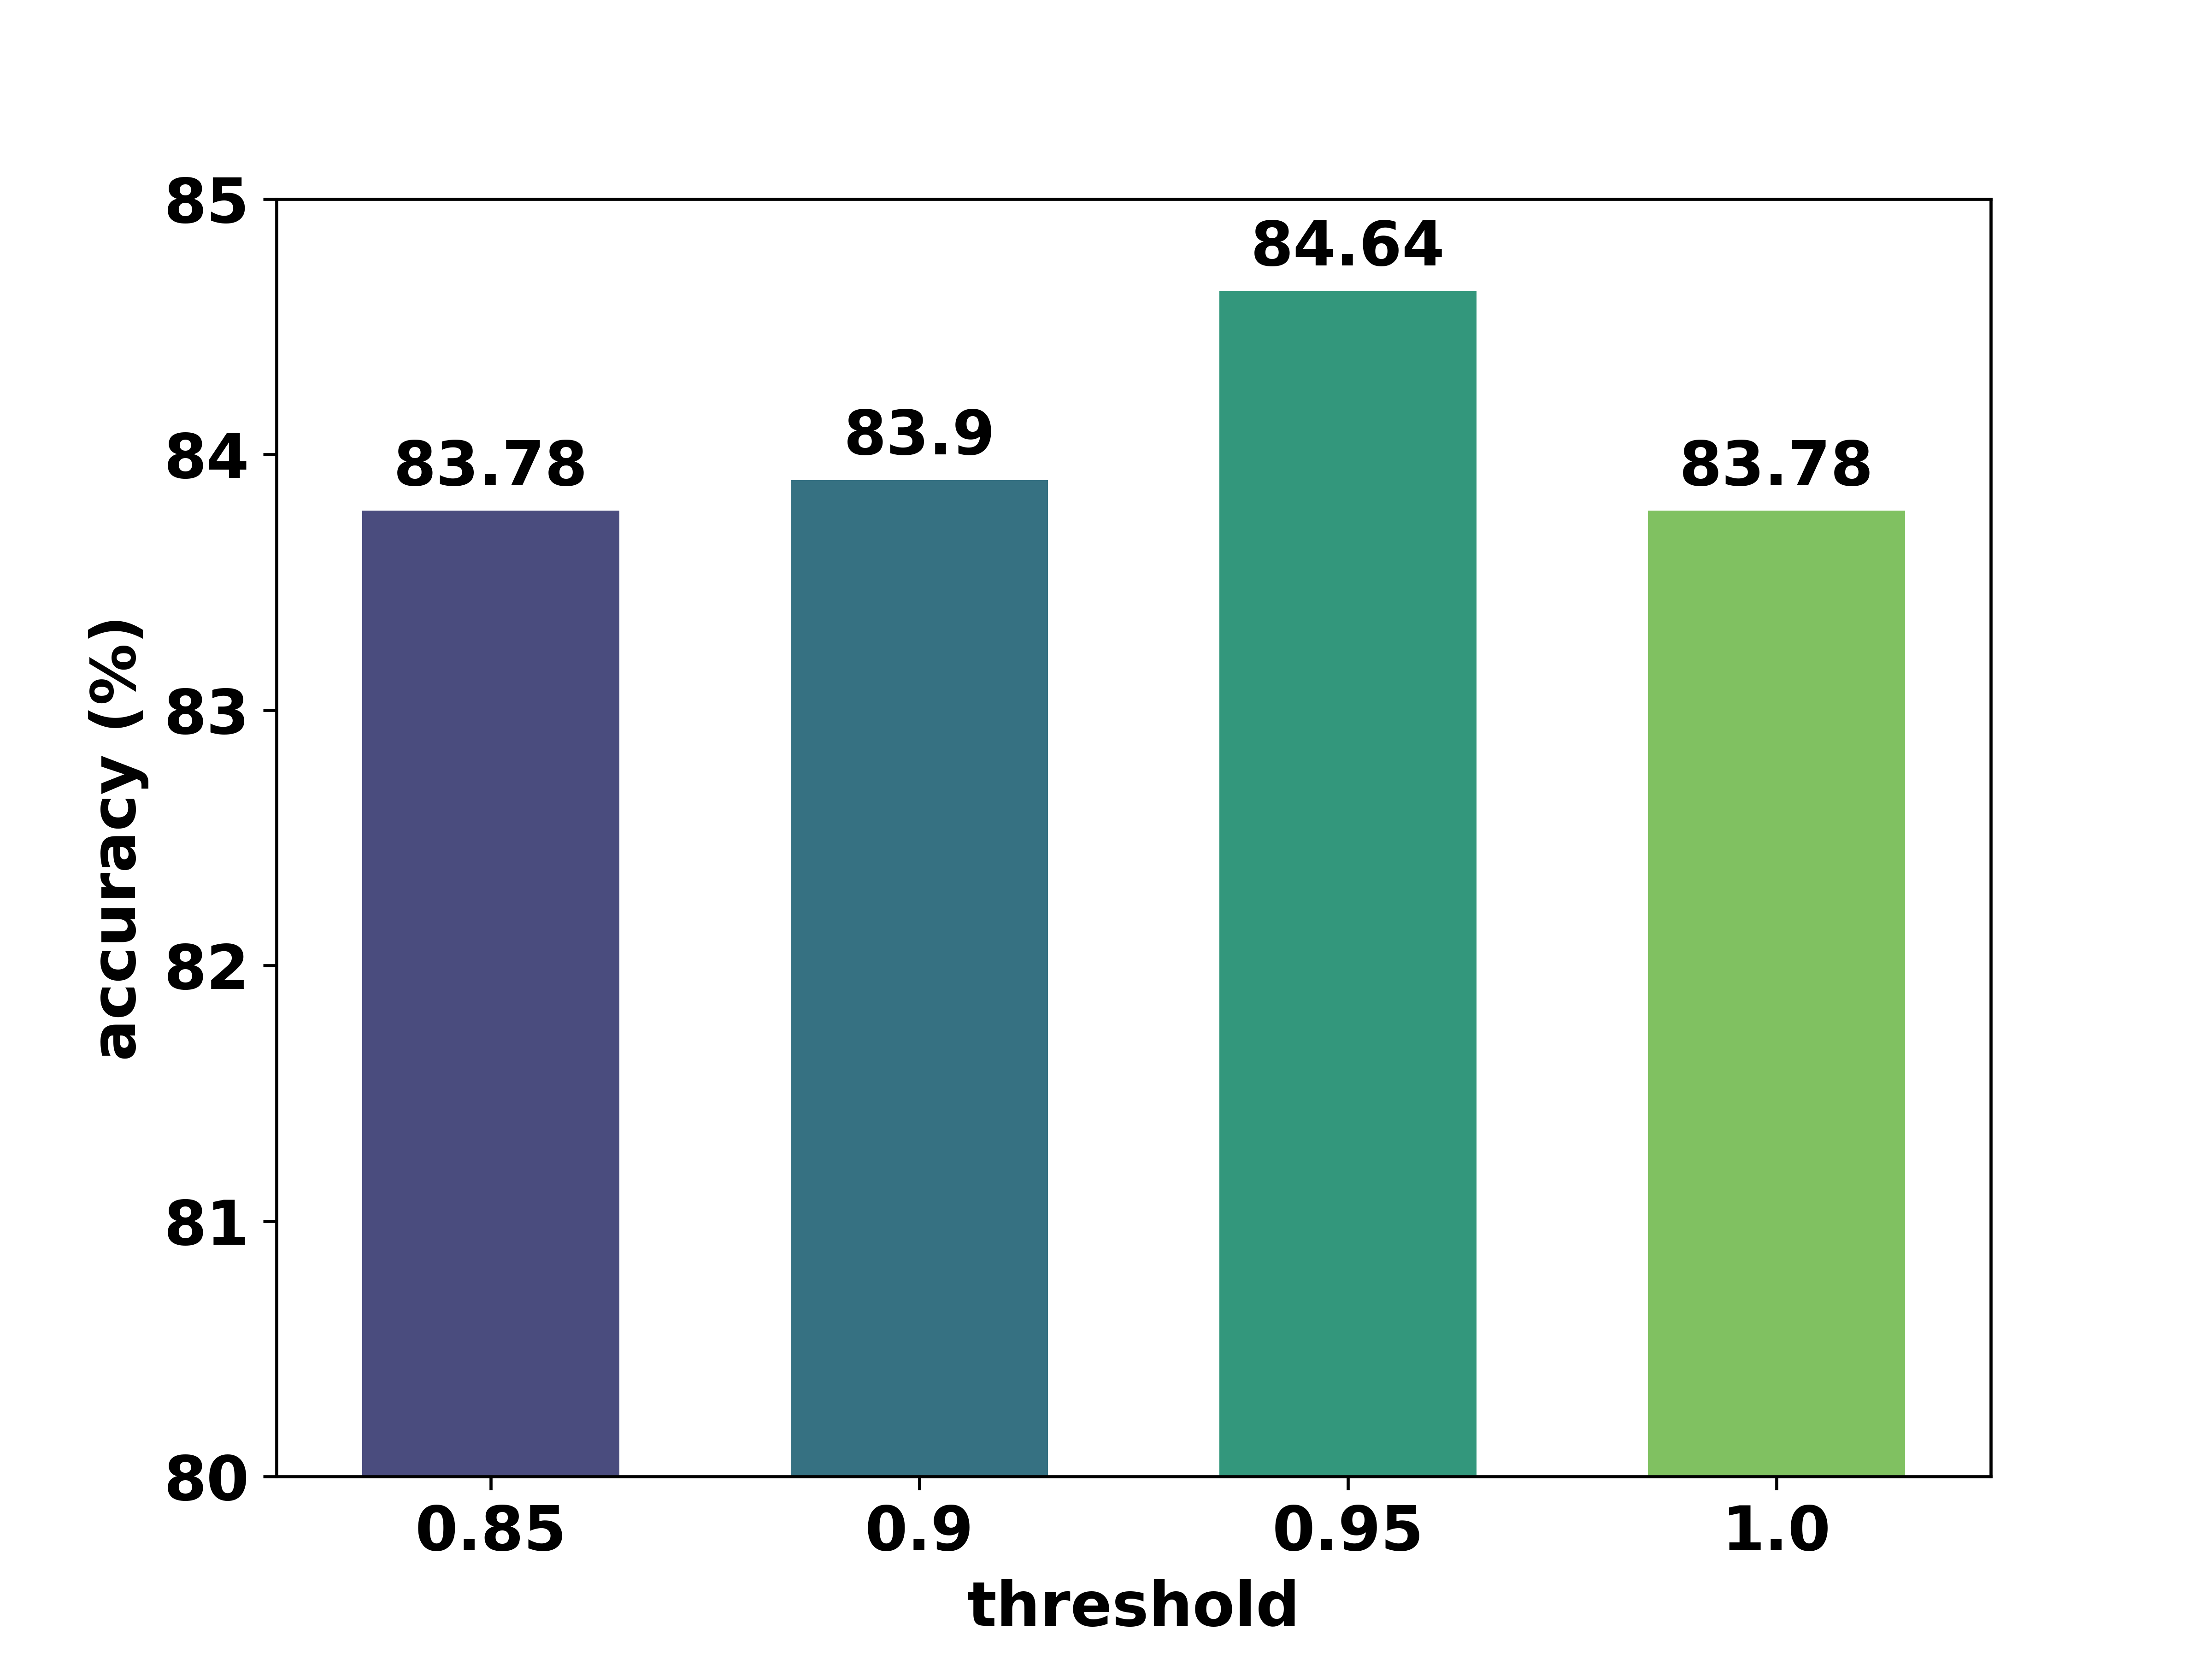
\includegraphics[width=\linewidth]{FIGURES/rlpl/accuracy_vs_threshold.png}
    \caption{Effect of the pseudo labels threshold, $\tau$.}
    \label{fig:threshold}
\end{subfigure}
\caption{Effects of different hyperparameters on model performance.}
\end{figure}

We conduct extensive ablation studies to evaluate the effectiveness of our method against the PL algorithm with random initialization and RLPL without PLs. Results in Table \ref{table:ablation} demonstrate the consistent superiority of RLPL across diverse datasets and label regimes. The PL with random initialization exhibits limited performance, particularly struggling with low-label scenarios (e.g., 30.49\% and 11.19\% accuracy with 250 labels), highlighting the importance of proper initialization for PL's reliability. 

RLPL without pseudo labeling shows substantial improvements over the baseline, achieving gains on STL-10 (83.20\% vs 53.34\%) and SVHN (71.25\% vs 11.19\%), validating the effectiveness of our representation learning strategy. The full RLPL framework, integrating both representation learning and pseudo labeling, consistently achieves the highest performance across all configurations, with particularly strong improvements in low-label settings (e.g., 48.93\% on CIFAR-10 with 250 labels, an 18.44\% improvement). This comprehensive performance advantage is reflected in the average accuracy across all settings, demonstrating RLPL's robust capability, especially in label-scarce scenarios where traditional approaches typically falter.

\subsection{Ablation on Noisy Teacher}

\begin{table}[!htbp]
\centering
\begin{tabular}{cc}
\hline
\textbf{Method} & \textbf{Accuracy (\%)} \\
\hline
Noisy Student    & 84.54 $\pm$ 0.05 \\
Noiseless Teacher & 84.59 $\pm$ 0.02 \\
Noisy Teacher     & 84.63 $\pm$ 0.02 \\
\hline
\end{tabular}
\caption{Input types ablation for pseudo labeling.}
\label{table:noise}
\end{table}
We investigate the impact of noisy samples (weakly augmented) in both teacher and student networks. Table~\ref{table:noise} shows the average performance of five different runs for three configurations: the noisy student, the noiseless teacher, and our proposed noisy teacher method. While the differences are subtle, they reveal interesting patterns in model behavior. The noisy student achieves 84.54\% accuracy with a standard deviation of 0.05, suggesting some variability in performance. When we remove noisy samples from the teacher network, we observe a marginal improvement to 84.59\% with reduced variance. Our proposed approach achieves the highest accuracy at 84.63\% with consistently low variance. These results suggest that weak augmentation in the teacher network inputs can provide additional regularization benefits.


% \subsection{Projector Dimensionality}
\subsection{Parameter Studies}

We conduct parameter sensitivity studies to examine the impact of key hyperparameters on RLPL's performance, focusing on the auxiliary loss weight and pseudo-label threshold. These studies help validate our design choices and provide insights for optimal configuration.

\subsubsection{Weight of the Auxiliary Loss}

We modify the weight of auxiliary loss, $\lambda$, from $0.25$ to $1.0$ with an increment of $0.25$. We observe that there is a strong effect of the weight on model performance. For weights other than $0.50$, the test accuracy declines as we move further from this value. The outputs are shown in Figure \ref{fig:weight}.

\subsubsection{Threshold for Pseudo Labels}

We vary the threshold, $\tau$, from $0.85$ to $1.0$ with an increment of $0.05$. We observe that the highest accuracy is obtained at $0.95$, and it keeps decreasing for a lower threshold value. Again, the accuracy decreases for a threshold value of $1.0$. For any threshold other than $0.95$, the accuracy drops below 84.0\%. The outputs are shown in Figure \ref{fig:threshold}.

\subsection{Conclusion}

We present RLPL, a novel semi-supervised learning framework that maximizes unlabeled data utility while addressing limitations in existing methods. RLPL achieves consistent improvements over SOTA methods with smaller batch sizes, enhancing efficiency in memory-constrained environments. Our experiments demonstrate substantial performance gains across multiple datasets, particularly with limited labeled data. RLPL also shows exceptional transferability across diverse downstream classification tasks without requiring pseudo labels for adaptation. These advantages in data efficiency, robustness, and generalization make RLPL particularly valuable for applications demanding memory efficiency and cross-task adaptability.

\section{Overall Findings}

In this chapter, we have explored maximizing unlabeled data utility in machine learning through advanced semi-supervised learning techniques, with particular focus on their role in enabling practical wireless foundation models. Our investigation has yielded several important findings that contribute to both theoretical understanding and practical application of SSL methods in the context of our three-stage foundation model framework.

\textbf{Fundamental limitations identified:} Existing representation learning approaches depend on large batch sizes and fail to effectively leverage unlabeled data during downstream tasks. These limitations create barriers to deployment in resource-constrained wireless environments and prevent full utilization of the abundant unlabeled signals available in spectrum monitoring scenarios. For wireless foundation models, these constraints are particularly critical since edge deployment often involves limited computational resources.

\textbf{RLPL framework contributions:} Our proposed RLPL (Representation Learning with Pseudo-Labeling) framework addresses these limitations through a two-phase approach combining improved representation learning with meta-pseudo-labeling. The key innovation in the representation learning phase is incorporating auxiliary loss functions that extract additional information from each training sample, enabling stable learning even with smaller batch sizes. This demonstrates that effective representation learning need not depend on massive computational resources—critical for wireless foundation model deployment on resource-constrained hardware.

The meta-pseudo-labeling component further enhances model performance by creating a feedback loop between teacher and student networks, significantly improving pseudo-label quality in low-supervision regimes where traditional pseudo-labeling methods struggle. For wireless signals, where obtaining expert annotations for every modulation scheme across all SNR conditions is prohibitively expensive, this capability to learn from high-quality pseudo-labels is essential. By combining strong initialization from representation learning with refined pseudo-label generation, RLPL creates a synergistic effect that maximizes information extraction from unlabeled data.

\textbf{Experimental validation:} Extensive evaluation confirms that RLPL consistently outperforms state-of-the-art methods across diverse datasets and supervision levels. Performance improvements are most pronounced in extremely label-scarce scenarios (e.g., CIFAR-10 with only 250 labels, achieving up to 15.74\% accuracy gains), directly relevant to wireless scenarios where collecting labeled modulation data at scale is impractical. Additionally, RLPL demonstrates excellent transferability across heterogeneous downstream tasks without requiring task-specific adaptations—aligning with the foundation model principle of learning general-purpose representations that transfer broadly.

\textbf{Robustness and ablation insights:} Parameter sensitivity studies reveal that RLPL's performance is robust across a range of hyperparameter values, with optimal configurations for the auxiliary loss weight ($\lambda=0.5$) and pseudo-label threshold ($\tau=0.95$) providing consistent improvements. Ablation studies confirm that both components contribute meaningfully to final performance, with their combination yielding the strongest results.

\textbf{Foundation model implications:} This chapter demonstrates how semi-supervised learning serves as a critical enabling methodology for wireless foundation models. RLPL allows Stage 1 (self-supervised pre-training, Chapter 2) to operate effectively with minimal labeled data by maximizing unlabeled signal utilization. It enhances Stage 2 (meta-learning adaptation, Chapter 3) by providing high-quality pseudo-labeled samples that augment few-shot learning episodes. Together, these capabilities address the fundamental data bottleneck in wireless AI: abundant unlabeled signals but scarce expert annotations.

The demonstrated performance gains suggest that SSL approaches like RLPL can significantly reduce annotation requirements while maintaining high model accuracy, addressing a critical bottleneck in deploying wireless foundation models at scale. By enabling effective learning from limited labels and abundant unlabeled data, RLPL makes the three-stage foundation model framework practical for real-world wireless applications.

\textbf{Pathway forward:} The principles and techniques presented in this chapter provide a foundation for developing more data-efficient, accessible wireless foundation models capable of operating effectively with varying levels of supervision. With Stages 1-2 (pre-training + adaptation) now established through Chapters 2-4, the next chapter (Chapter 5) completes our vision by integrating these learned representations with large language models to enable true open-set recognition—moving beyond closed-set classification to general-purpose wireless intelligence.

